% This text is proprietary.
% It's a part of presentation made by myself.
% It may not used commercial.
% The noncommercial use such as private and study is free
% Sep. 2005 
% Author: Sascha Frank 
% University Freiburg 
% www.informatik.uni-freiburg.de/~frank/


\documentclass[aspectratio=169]{beamer}


%%% HANDOUT START
%  \documentclass[11pt,handout,aspectratio=169]{beamer}
%  \usepackage{pgfpages}
%  \pgfpagesuselayout{6 on 1}[a4paper]
%  \setbeamertemplate{footline}{% set footline options
%   $\qquad\qquad$\insertpagenumber   
%   }

 
%%% HANDOUT END

\usefonttheme{professionalfonts}
 
%\setbeamertemplate{page number in head/foot}[totalframenumber]
%\beamertemplatenavigationsymbolsempty

%\setbeamerfont{page number in head/foot}{size=\footnotesize}


%pdfnup --a4paper --keepinfo --nup 1x3 --frame true   --scale 0.92 --no-landscape --outfile handout.pdf slides.pdf


\setbeamercovered{transparent=10}


\usepackage{multirow}
% \usepackage{pgfpages}
% \mode<handout>{\setbeamercolor{background canvas}{bg=black!5}}
% \pgfpagesuselayout{4 on 1}[letterpaper,border shrink=2mm]

%\documentclass[handout]{beamer}
% \setbeamertemplate{bibliography entry title}{}
% \setbeamertemplate{bibliography entry location}{}
% \setbeamertemplate{bibliography entry note}{}
\setbeamertemplate{bibliography item}{\insertbiblabel}

\newcommand{\Prob}{{\rm I\hspace{-0.8mm}P}}

\newcommand{\p}[0]{\mathbf{p}}
\newcommand{\q}[0]{\mathbf{q}}

\newcommand{\e}[0]{\textbf{e}}
\newcommand{\PP}[0]{\mathbf{P}}
\newcommand{\II}[0]{\textbf{I}}
\newcommand{\Q}[0]{\mathbf{Q}}
\newcommand{\E}[0]{\mathbb{E}}
\newcommand{\X}[0]{\textbf{X}}
\newcommand{\Z}[0]{\textbf{Z}}
\newcommand{\s}[0]{\mathbf{s}}
\newcommand{\C}[0]{\textbf{C}}
\newcommand{\es}[0]{\mathbf{s}}
\newcommand{\trev}[0]{\overleftarrow}
\definecolor{mygray}{gray}{0.6}
\newcommand{\diag}{\mathbf{diag}}
\newcommand{\iii}[0]{\mathbf{i}}

%\dual to oznacznie dualnosci, oryginalnie *
%\newcommand{\dual}[0]{\circledast}
\newcommand{\dual}[0]{*}

%\monD to oznacznie tej drugiej monotonicznosci, czyli np. ^\monD-Mobius monotonicity
%\newcommand{\monD}[0]{\lozenge}
\newcommand{\monD}[0]{\downarrow}
\newcommand{\monU}[0]{\uparrow}

\usepackage{cancel} 

\usepackage{dsfont}
 
\newcommand{\indic}[0]{\mathds{1}}
\usepackage{pdfpages}
\usepackage{graphicx}
\usepackage{soul} 
\usepackage{tikz}
\usepackage[utf8]{inputenc}
\usepackage[T1]{fontenc}
\usetikzlibrary{arrows}




\setbeamertemplate{theorems}[numbered]

% Add support for \subsubsectionpage
%\def\subsubsectionname{\translate{Subsubsection}}
%\def\insertsubsubsectionnumber{\arabic{subsubsection}}
% \setbeamertemplate{subsubsection page}
% {
%   \begin{centering}
%     {\usebeamerfont{subsubsection name}\usebeamercolor[fg]{subsubsection name}\subsubsectionname~\insertsubsubsectionnumber}
%     \vskip1em\par
% %     \begin{beamercolorbox}[sep=4pt,center]{d part title}
% %       \usebeamerfont{subsubsection title}\insertsubsubsection\par
% %     \end{beamercolorbox}
%   \end{centering}
% }
% \def\subsubsectionpage{\usebeamertemplate*{subsubsection page}}


\AtBeginSection{\frame{\sectionpage}}
\AtBeginSubsection{\frame{\subsectionpage}}
\AtBeginSubsubsection{\frame{\subsubsectionpage}}
 
\usepackage{tikz}

\usepackage{pgfplots}
\pgfplotsset{compat=1.11}
 

 % FROM BOOK:
 


\usepackage{algorithm}

\usepackage{algpseudocode}
\usepackage{caption}
\usepackage{comment}
\usepackage{booktabs}


 \usepackage[T1]{fontenc}
%\usepackage[utf8]{inputenc}
%\usepackage[polish]{babel}

\usepackage{tikz}
\usetikzlibrary{arrows}
\usetikzlibrary{arrows.meta}
\usetikzlibrary{patterns}
%\usetikzlibrary{decorations.pathreplacing,calligraphy}
\usetikzlibrary{decorations.text}
\usetikzlibrary{decorations.markings}
\usetikzlibrary{decorations.pathreplacing}
\usetikzlibrary{arrows.meta,babel}
\usetikzlibrary{shapes.misc}

\usepackage{pgfplots}
%\pgfplotsset{compat=1.7}
\pgfplotsset{compat=1.16}
%\pgfplotsset{compat=1.18}
\usepgfplotslibrary{fillbetween}

\usepackage{subfig}

\usepackage{etoolbox}


% 2. Configuration Commands
% ============================
% Code listings (for \begin{lstlisting}...\end{lstlisting})
\usepackage{listings}
\lstset{
  basicstyle=\ttfamily\footnotesize,
  columns=fullflexible,
  keepspaces=true,
  showstringspaces=false,
  frame=none,
  numbers=none,
  breaklines=true,
}
%
% \renewcommand{\lstlistingname}{Python Listing} % Listing -> Algorithm
% \lstset{basicstyle=\fontsize{8}{12}\selectfont\ttfamily}
% \lstset{language=Python}
%
% \captionsetup[figure]{font=small} % Changes font size in figure captions
%
% \captionsetup[algorithm]{font=normal} % Changes font size in algorithm captions
% \AtBeginEnvironment{algorithmic}{\normalsize} % Changes font size inside algorithm body
%


% --- Bold (\bf) Commands ---


\newcommand{\bfM}{\mathbf{M}}
\newcommand{\bfU}{\mbox{\boldmath $U$}}
\newcommand{\bfu}{\mbox{\boldmath$u$}}
\newcommand{\bfv}{\mathbf{v}}
\newcommand{\bfw}{\mathbf{w}}
\newcommand{\bfx}{\mathbf{x}}
\newcommand{\done}{\textbf{\textcolor{red}{DONE }}}
\newcommand{\bfy}{\mbox{\boldmath$y$}}
\newcommand{\bfz}{\mathbf{z}}
\newcommand{\bfg}{\mbox{\boldmath$g$}}
\newcommand{\bfh}{\mbox{\boldmath$h$}}
\newcommand{\bfb}{\mbox{\boldmath$b$}}
\newcommand{\bfp}{\mathbf{p}}
\newcommand{\bfq}{\mathbf{q}}
\newcommand{\bfJ}{\mbox{\boldmath $J$}}
\newcommand{\bfP}{\mathbf{P}}
%\newcommand{\bfT}{\mbox{\boldmath $T$}}
\newcommand{\bfT}{\vec{T}}
\newcommand{\bfL}{\mathbf{L}}
\newcommand{\bfm}{\mbox{\boldmath$m$}}

\newcommand{\bfSigma}{\boldsymbol{\Sigma}}
\newcommand{\bfsigma}{\mbox{\boldmath $\sigma$}}
\newcommand{\bfmu}{\mbox{\boldmath $\mu$}}
\newcommand{\bfzero}{{\bf 0}}


\newcommand{\bfa}{\boldsymbol{a}}
\newcommand{\bfA}{\mathbf{A}}
\newcommand{\bfB}{\mathbf{B}}
\newcommand{\bbX}{\mathbb{X}}
\newcommand{\bfX}{\mathbf{X}}
\newcommand{\bfY}{\mathbf{Y}}
\newcommand{\bfZ}{\mathbf{Z}}
\newcommand{\bfV}{\mbox{\boldmath $V$}}
\newcommand{\bfC}{\mathbf{C}}
\newcommand{\bbR}{\mathbb{R}}
\newcommand{\bbN}{\mathbb{N}}
\newcommand{\bbZ}{\mathbb{Z}}
\newcommand{\bfS}{\mathbf{S}}
\newcommand{\bfD}{\mathbf{D}}
\newcommand{\bff}{\mathbf{f}}
\newcommand{\bfF}{\mathbf{F}}
\newcommand{\bfI}{\mathbf{I}}
\newcommand{\bfe}{\mathbf{e}}
\newcommand{\bfk}{\mbox{\boldmath$k$}}
\newcommand{\bfn}{\mbox{\boldmath$n$}}
\newcommand{\bfR}{\mathbf{R}}
\newcommand{\bfQ}{\mathbf{Q}}
\newcommand{\bfG}{\mbox{\boldmath $G$}}

\newcommand{\bfPi}{\mbox{\boldmath $\Pi$}}
\newcommand{\bfPhi}{\mbox{\boldmath $\Phi$}}
\newcommand{\bfPsi}{\mbox{\boldmath $\Psi$}}
\newcommand{\bfLambda}{\mbox{\boldmath $\Lambda$}}
\newcommand{\bflambda}{\mbox{\boldmath $\lambda$}}

\newcommand{\bfgamma}{\mbox{\boldmath $\gamma$}}
\newcommand{\bfalpha}{\mbox{\boldmath $\alpha$}}
\newcommand{\bfeta}{\mbox{\boldmath $\eta$}}
\newcommand{\bftheta}{\boldsymbol{\theta}}
\newcommand{\bfpi}{\mbox{\boldmath$\pi$}}
\newcommand{\bfnu}{\mbox{\boldmath $\nu$}}

\newcommand{\bft}{\mbox{\boldmath$t$}}


% --- Caligraphic (\cal) Commands ---

\newcommand{\calA}{{\cal A}}
\newcommand{\calE}{{\cal E}}
\newcommand{\calL}{{\cal L}}
\newcommand{\calM}{{\cal M}}
\newcommand{\calN}{{\cal N}}
\newcommand{\calF}{{\cal F}}
\newcommand{\calG}{{\cal G}}
\newcommand{\calD}{{\cal D}}
\newcommand{\calB}{{\cal B}}
\newcommand{\calH}{{\cal H}}
\newcommand{\calI}{{\cal I}}
\newcommand{\calP}{{\cal P}}
\newcommand{\calR}{{\cal R}}
\newcommand{\calQ}{{\cal Q}}
\newcommand{\calS}{{\cal S}}
\newcommand{\calT}{{\cal T}}
\newcommand{\calU}{{\cal U}}
\newcommand{\calC}{{\cal C}}
\newcommand{\calK}{{\cal K}}
\newcommand{\calX}{{\cal X}}
\newcommand{\calV}{{\cal V}}
\newcommand{\cals}{{\cal S}}

\newcommand{\ind}{\boldsymbol{1}}
\newcommand{\Exp}{\mathbb{E}}
\newcommand{\Var}{\mathbb{V}ar}


\newcommand{\eqdistr}{\stackrel{\cal D}{=}}
\newcommand{\convdistr}{\stackrel{\cal D}{\rightarrow}}
\newcommand{\convrel}{\stackrel{\cal D}{\sim}}
\newcommand{\convas}{\stackrel{\rm a.s.}{\rightarrow}}
\newcommand{\convprob}{\stackrel{\Pr}{\rightarrow}}


\begin{document}
 

\title{Introduction to simulations and Monte Carlo methods:
\\ Generating random variables}
\author{Pawe{\l} Lorek  \\ \textsl{Mathematical Institute, University of Wroc{\l}aw, Poland} \\
\ \\
}

%\author{AMS Special Session on Transient Probabilities of Random Processes, Duality Theory and Gambler’s Ruin Probabilities}

\date{\today}

\frame{\titlepage} 


% \section{Section 1}
% \subsection{Subsection 1}
% \frame{}\frame{}
% \subsection{Subsection 2}
% \subsubsection{Subsubsection 1}
% \frame{}
% \section{Section 2}
% \frame{}
% 

%\frame{\frametitle{Table of contents}\tableofcontents} 

% =======================
% PRNG — formal basics
% =======================

% \section{Pseudorandom numbers}
% % =======================
% % PRNG — formal basics
% % =======================
% % =======================
% % PRNG — formal basics
% % =======================
%
% \section{Pseudorandom number generators (PRNGs)}
% --- Generating random numbers: setup & inverse transform ---
\begin{frame}{Generating random numbers: setup \& inverse transform}
\textbf{Assumption.} We have access to a (pseudo)random variable \(U\sim\calU[0,1)\) on the computer.

\medskip
\textbf{Goal.} Generate a target random variable \(X\) with prescribed c.d.f.\ \(F_X\).

\medskip
\textbf{Inverse Transform Method.} If \(F_X\) is strictly increasing and continuous, then
\[
X \;=\; F_X^{-1}(U)\quad\Rightarrow\quad X\sim F_X .
\]
\pause
\smallskip
\textit{Proof.} For any \(x\in\mathbb{R}\),
\[
\Prob(X\le x)
= \Prob\!\big(F_X^{-1}(U)\le x\big)
=\Prob\!\big(F_X(F_X^{-1}(U))) \le F_X(x)\big)
= \Prob\!\big(U \le F_X(x)\big)
= F_X(x),
\]
since \(F_X\) is strictly increasing (so \(F_X^{-1}\) exists) and \(U\sim\calU[0,1)\).

\medskip \pause
\textbf{Algorithm.}
\begin{enumerate}
  \item Generate \(U\sim\calU[0,1)\).
  \item Set \(X=F_X^{-1}(U)\).
\end{enumerate}

\medskip
\textbf{Example (Exponential \(\lambda\)).} \(F_X(x)=1-e^{-\lambda x}\) for \(x\ge 0\).
Then \(F_X^{-1}(u)= -\tfrac{1}{\lambda}\ln(1-u)\), so \(X= -\tfrac{1}{\lambda}\ln(1-U)\), or $X=-{1\over \lambda}\ln(U)$ (since $U\stackrel{\mathcal{D}}{=}1-U$)
\end{frame}






\begin{frame}{Inverse Transform Method (ITM)}
We aim to generate a random variable \(X\) with cumulative distribution function (c.d.f.)
\(F(x)=\Prob(X\leq x)\) using the \textbf{Inverse Transform Method (ITM)}.
We employ \(U\sim\calU[0,1)\) as the source of randomness.

\medskip
\textbf{Generalized inverse function:}
\[
F^{\leftarrow}(u)=\inf\{x:\ u\le F(x)\}.
\]
If \(F\) is continuous and strictly increasing, \(F^{\leftarrow}\) is the usual inverse of \(F\).


\end{frame}



\begin{frame}{Inverse Transform Method (ITM)}

  \begin{tabular}{ccc}
 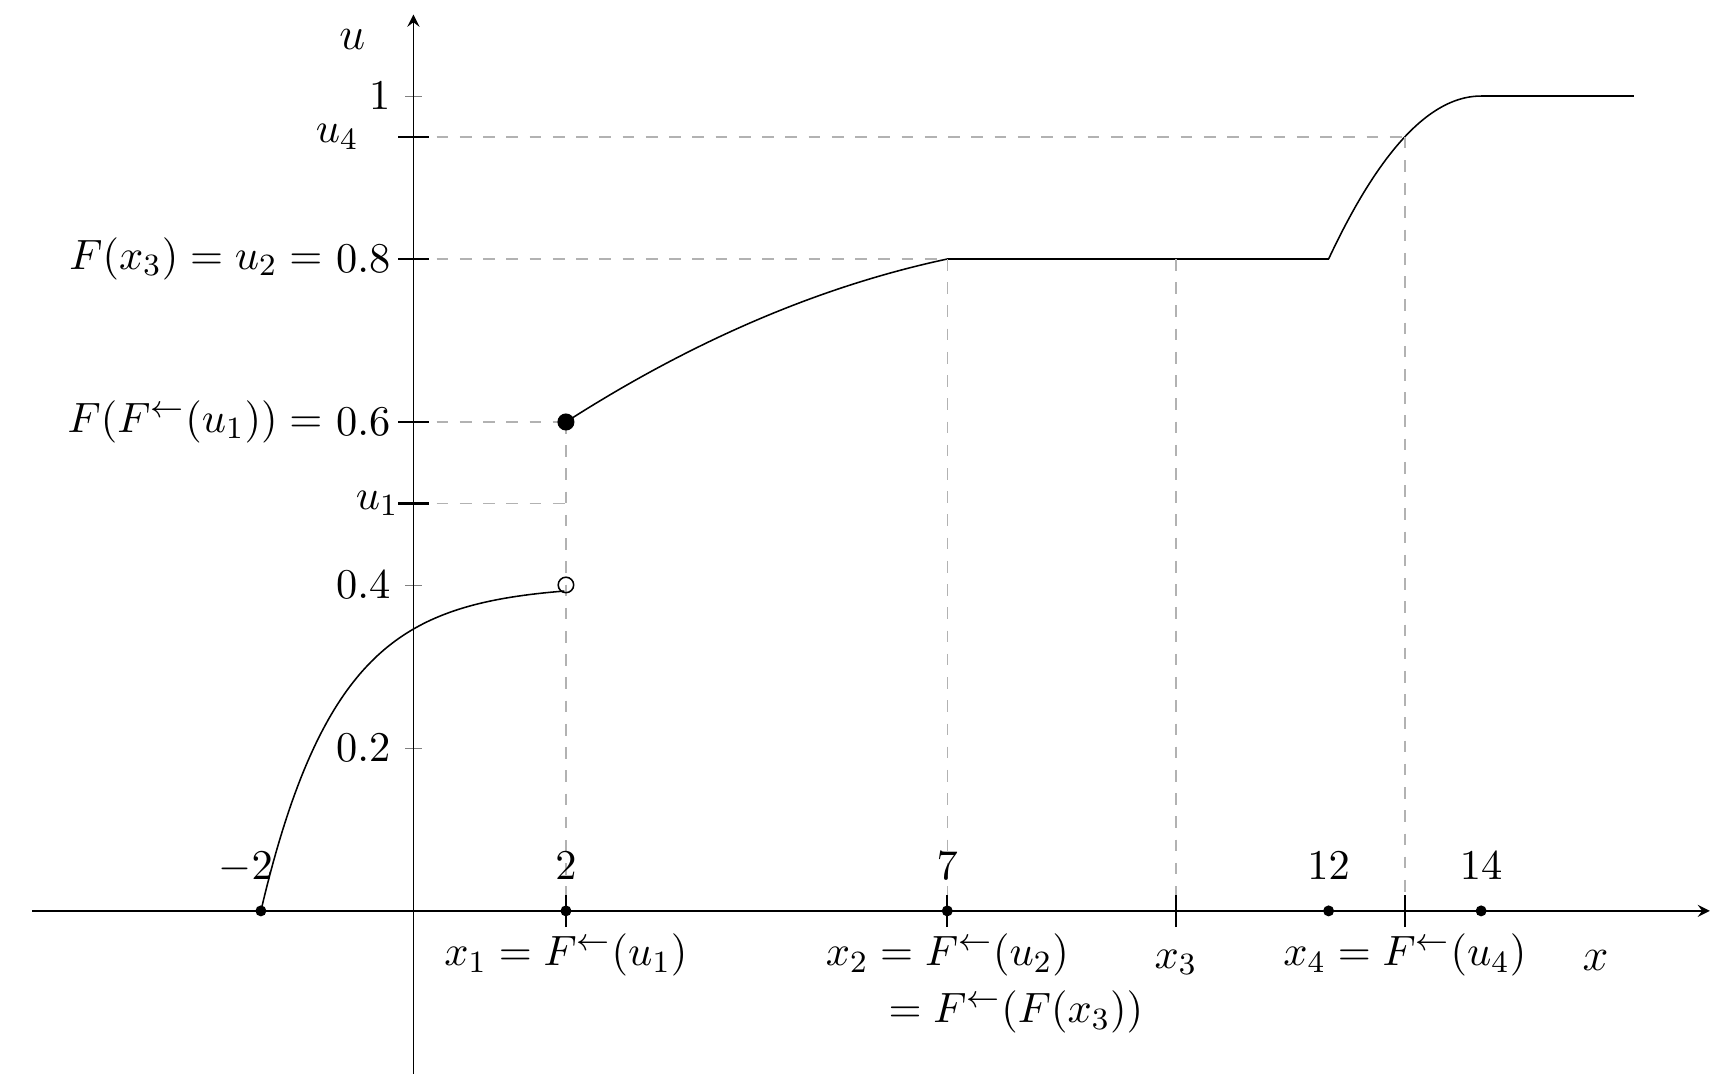
\includegraphics[width=0.5\linewidth]{pics/figure_inverse_fun1.png}
&
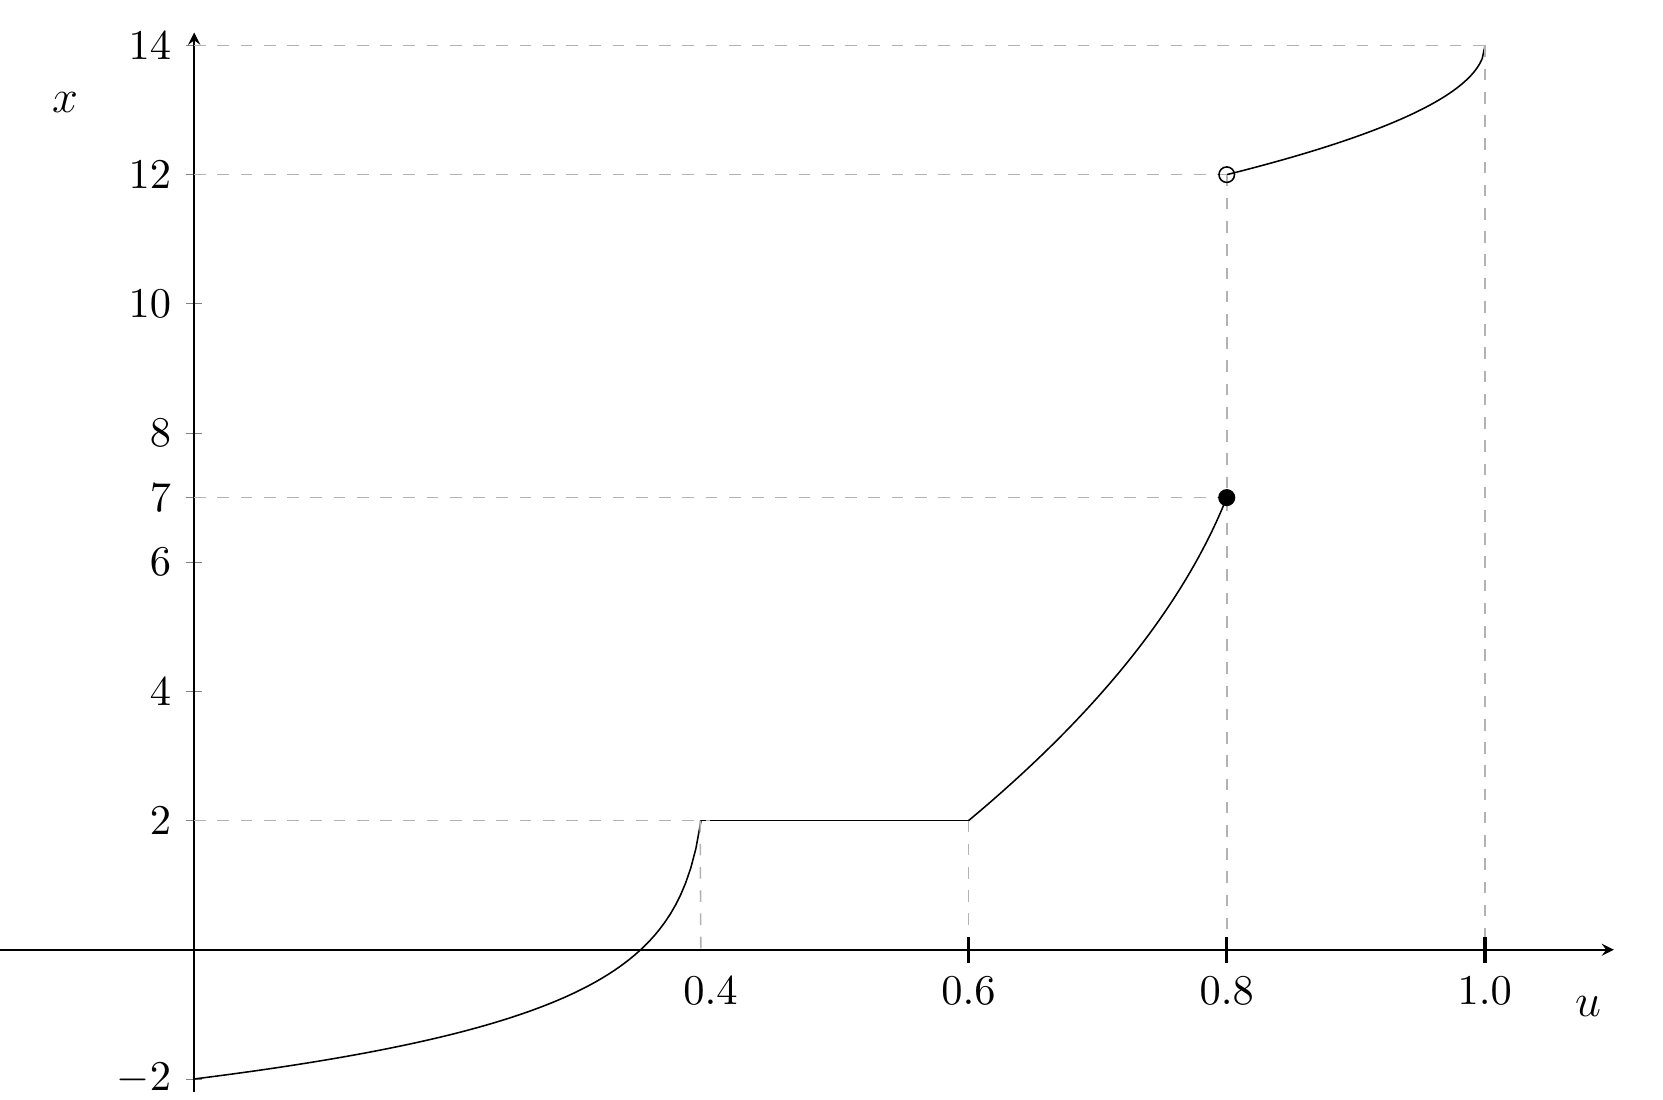
\includegraphics[width=0.45\linewidth]{pics/figure_inverse_fun2.png} \\
$F(x)$ & $F^{\leftarrow}(u)$
 \end{tabular}

\end{frame}



\begin{frame}{Inverse Transform Method (ITM)}

  \begin{tabular}{ccc}
 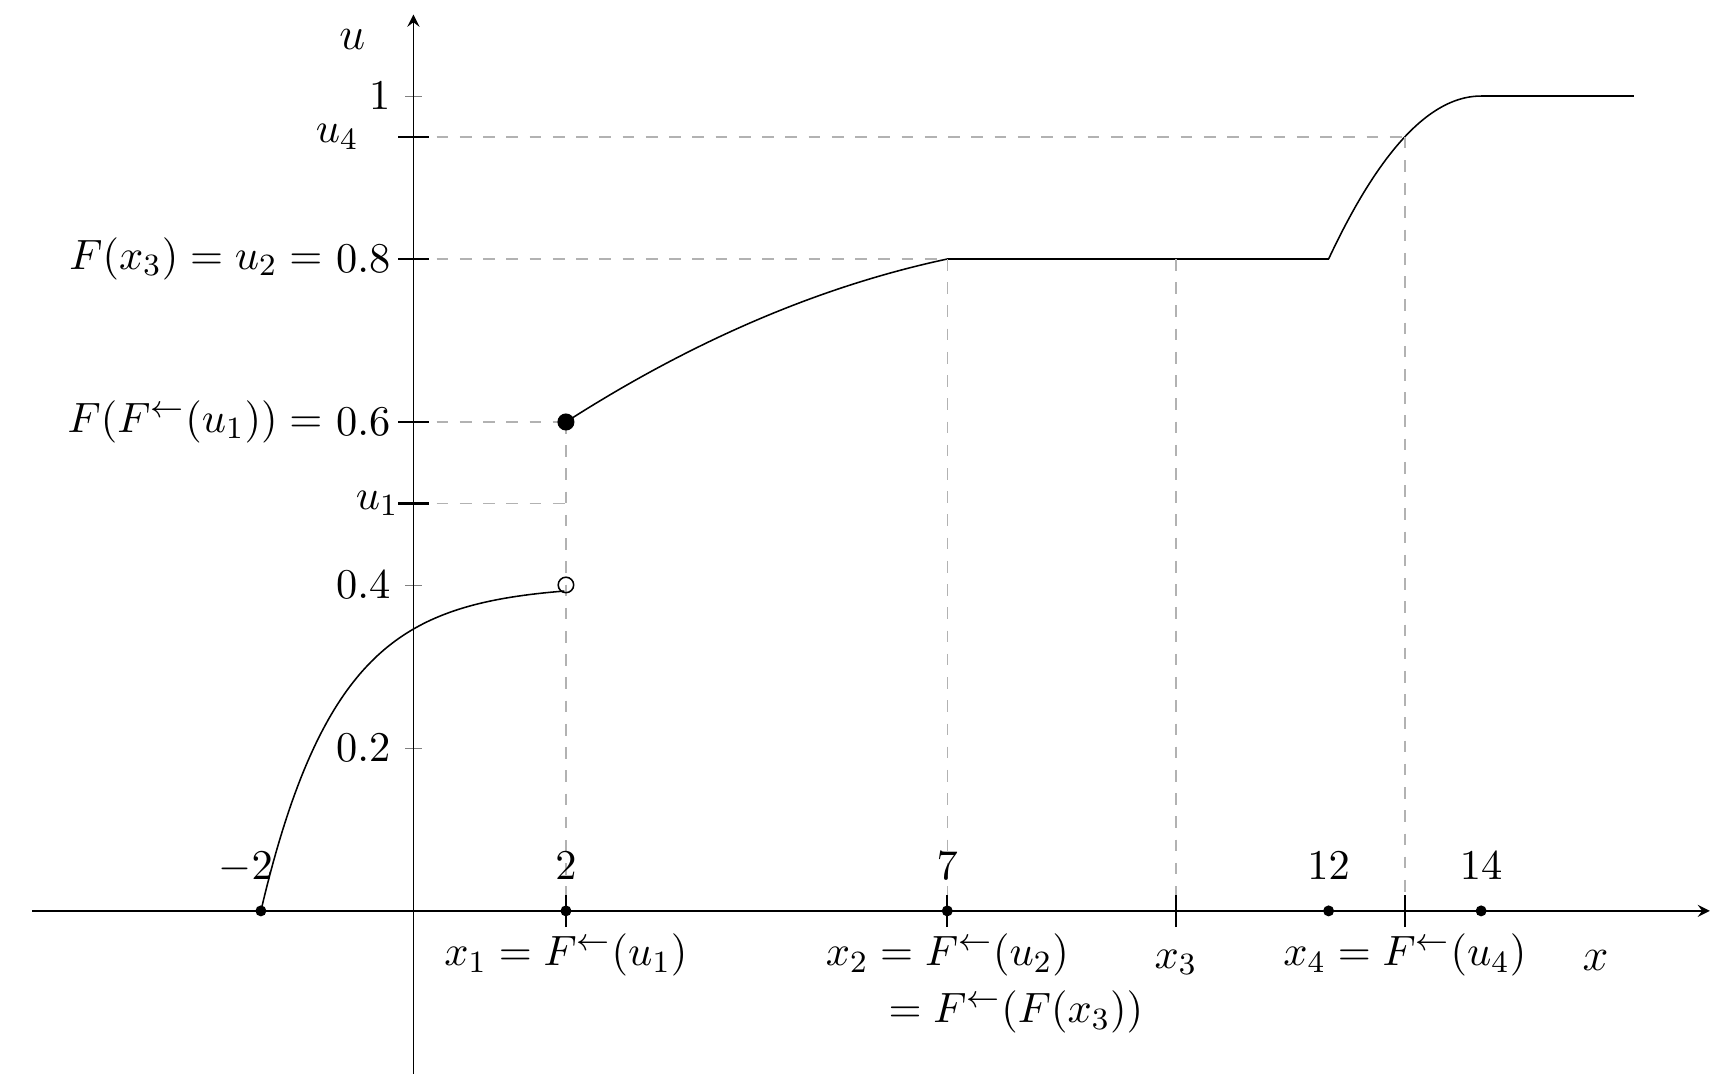
\includegraphics[width=0.5\linewidth]{pics/figure_inverse_fun1.png}
&
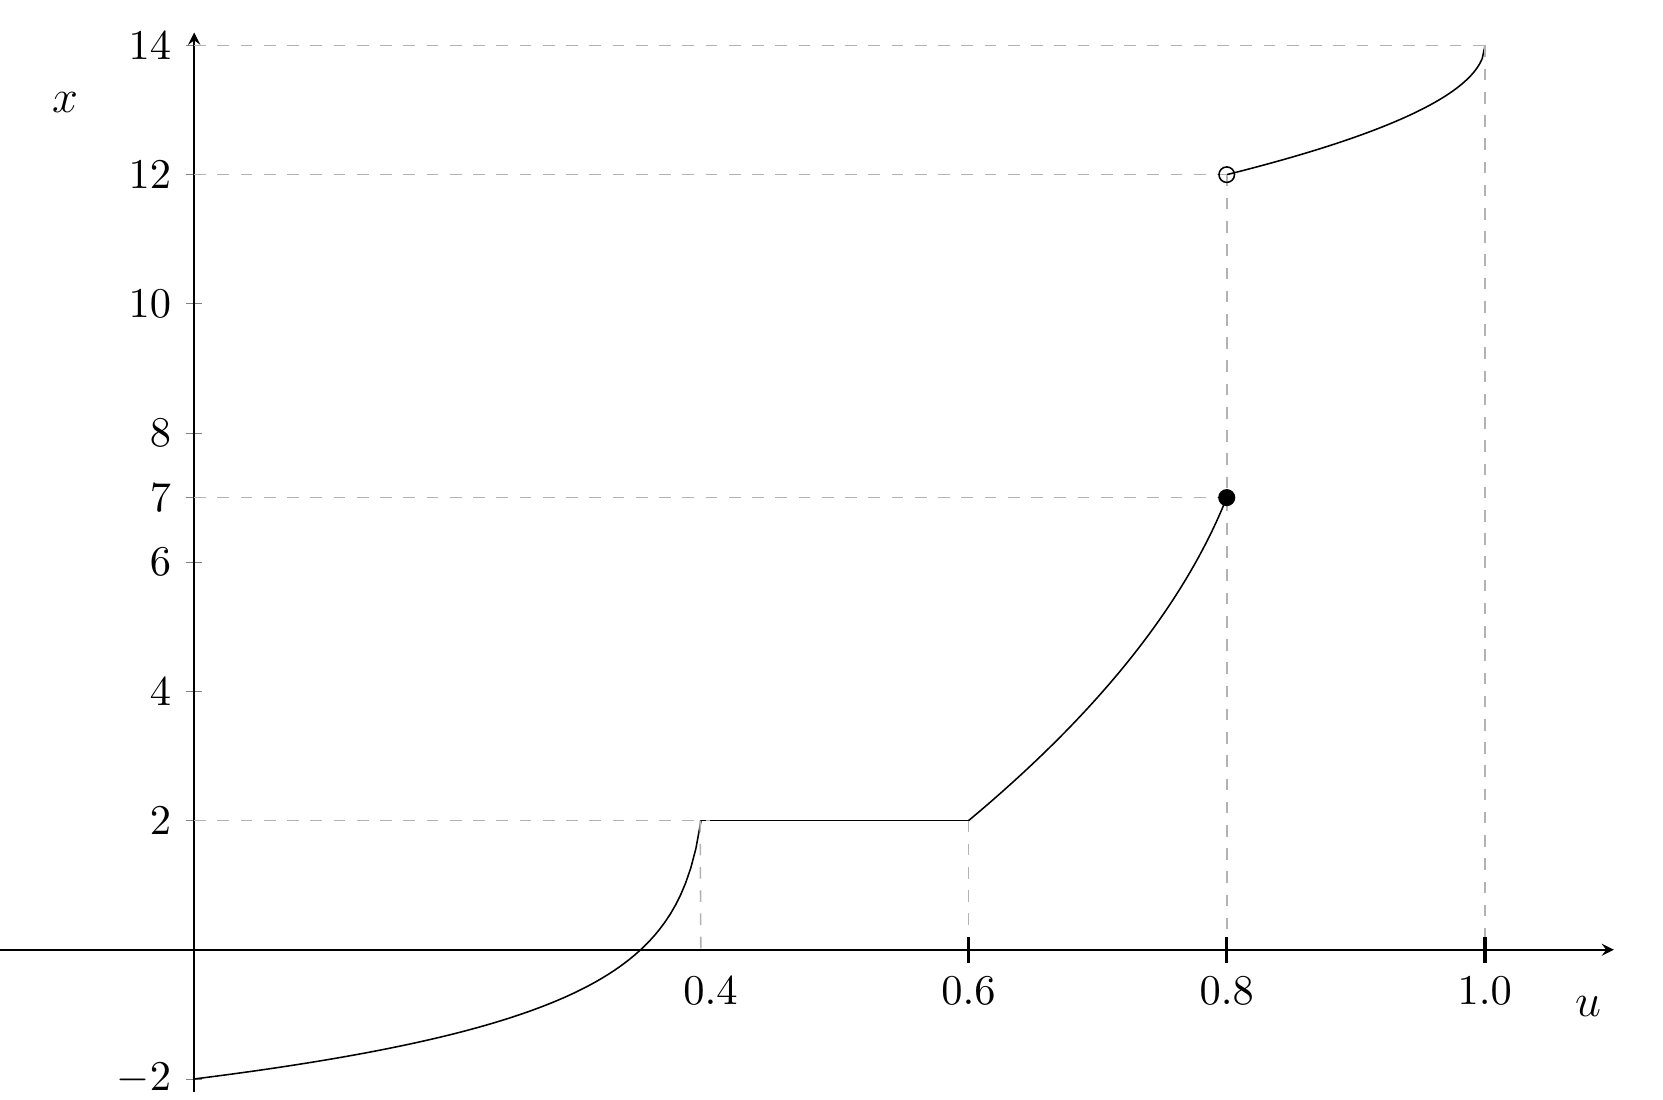
\includegraphics[width=0.45\linewidth]{pics/figure_inverse_fun2.png} \\
$F(x)$ & $F^{\leftarrow}(u)$
 \end{tabular}
 \begin{itemize}
 \item[(P1)] \(F^{\leftarrow}(u)\) is non-decreasing and left-continuous.
 \item[(P2)] If \(F\) is strictly increasing and \(u\in F(\bbR)\), then
       \(u=F(x)\) iff \(F^{\leftarrow}(u)=x\).
 \item[(P3)] If \(u\notin F(\bbR)\), it may happen that \(F^{\leftarrow}(u)=x\) but \(u<F(x)\).
 \item[(P4)] \(F^{\leftarrow}(u)=\inf\{x:u\le F(x)\}=\sup\{x:u>F(x)\}\).
 \item[(P5)] \(F^{\leftarrow}(F(x))\le x\) (equality for strictly increasing \(F\)).
 \item[(P6)] \(F(F^{\leftarrow}(u))\ge u\).
\end{itemize}
\end{frame}




\begin{frame}{Inverse Transform Method (ITM)}

  We will denote the {\it tail} of a c.d.f.\ $F(x)$ by
$$\overline{F}(x)=1-F(x).$$
For a tail distribution c.d.f.\ $\overline{F}$, define
\begin{eqnarray*}
  \overline{F}^{\leftarrow}(u)&=&\inf\{x: \overline{F}(x)\le u\}\\
  &=&\inf\{x: 1-u\le F(x)\}={F}^{\leftarrow}(1-u).
\end{eqnarray*}

\end{frame}





\begin{frame}{Inverse Transform Method (ITM)}

 \begin{myLemma}\label{l:wlasnosci}
 The generalized inverse function $F^{\leftarrow}(u)$ has the following properties:
 \begin{enumerate}
      \item[a)] $u\le F(x)$ if and only if $F^{\leftarrow}(u)\le x$.
     \item[b)] If $F(x)$ is continuous, then $F(F^{\leftarrow}(u))=u$.
 \end{enumerate}
  \end{myLemma}

\textsl{Proof.}
 (a) See Fig. again:
 \par
 \begin{center}
 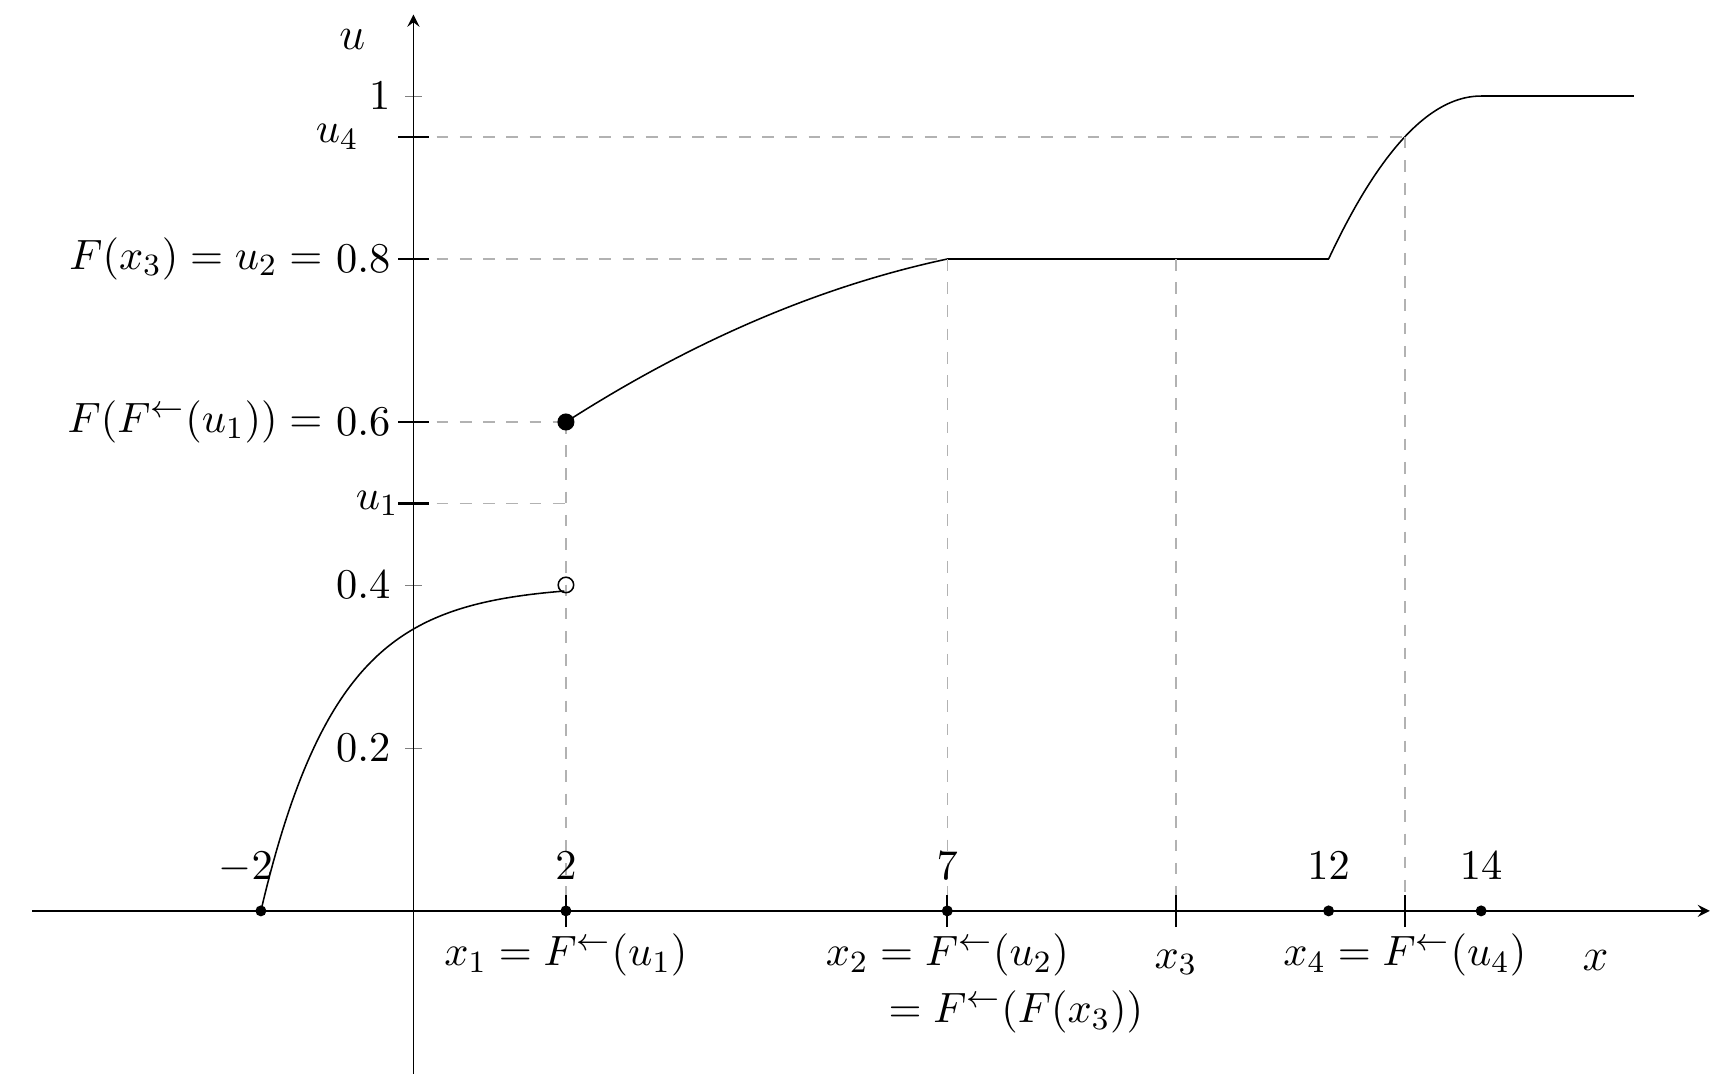
\includegraphics[width=0.65\linewidth]{pics/figure_inverse_fun1.png}
 \end{center}

\end{frame}



\begin{frame}{Inverse Transform Method (ITM)}
Part (b): If $F(x)$ is continuous, then $F(F^{\leftarrow}(u))=u$.
\bigskip\par
 We always have $F(F^{\leftarrow}(u))\ge u$, see property (P6).
On the other hand, take any $u\in(0,1)$ and let  $x$ be such that $u=F(x)$ (we can always find such $x$
because $F$ is continuous).
Notice the relationship $F^{\leftarrow}(u)\le x$.
Hence
$$ F(F^{\leftarrow}(u))\le F(x)=u,$$
which completes the proof of part  (b).

\end{frame}




\begin{frame}{Inverse Transform Method (ITM)}

 \begin{myProp}\label{p.ITM}
The following statements hold:
\begin{enumerate}
    \item Suppose $U$ is a uniformly distributed random variable. Then $F^{\leftarrow}(U)$ is a random variable with the distribution  $F$.
    \item If $F$ is continuous and  $X\sim F$, then $F(X)$ has the uniform distribution  $\calU[0,1)$.
\end{enumerate}
\end{myProp}

\begin{proof}
1. From Lemma \ref{l:wlasnosci} (a) we have
$$\Prob(F^{\leftarrow}(U)\le x)=\Prob(U\le F(x))=F(x)\;.$$
\pause
\newline 2. From Lemma \ref{l:wlasnosci} (a) we have
$$\Prob(F(X)\ge u)=\Prob(X\ge F^{\leftarrow}(u))\;.$$
Since a random variable $X$ has a continuous c.d.f., so it is atomless,
we can thus write
$$\Prob(X\ge F^{\leftarrow}(u))=\Prob(X> F^{\leftarrow}(u))=1-F(F^{\leftarrow}(u))\;,$$
which by virtue of Lemma \ref{l:wlasnosci} (b) is equal to $1-u$.
\end{proof}

\end{frame}





\begin{frame}{Inverse Transform Method (ITM)}
 \begin{myCor}\label{cor:p-value-uniform}
 Let the c.d.f.\ $F$ of $T$ be continuous. Then, the $p$-value has
 the uniform $\mathcal{U}[0,1)$ distribution.
\end{myCor}

\begin{proof}
As usual $U\sim\calU[0,1)$.
There are three scenarios for the $p$-value
\begin{itemize}
 \item \textbf{One-sided, right-tail}
In this case
$p$-value
$$p= 1-F(T) \stackrel{\textrm{Prop.~\ref{p.ITM} (b)}}{=}1-U\stackrel{\mathcal{D}}{=}U.$$
\pause
\item \textbf{One-sided, left-tail}\par
$$p= F(T) \stackrel{\textrm{Prop.~\ref{p.ITM} (b)}}{=}U.$$
\pause
\item \textbf{Two-sided, symmetric}
In this case, the distribution of $T$ is
$$F_{|T|}(t)=\Prob(-t\le T\le t) \stackrel{\textrm{continuity of } F}=\Prob(-t< T\le t)=F(t)-F(-t),$$
which is continuous. Hence
\[p=F_{|T|}(|T|) \stackrel{\textrm{Prop.~\ref{p.ITM} (b) }}{=}U. \]

\end{itemize}

\end{proof}

\end{frame}



\begin{frame}{Inverse Transform Method (ITM)}

\begin{algorithm}[H]
\caption{ITM; generating $X\sim F$}
\label{alg:genX}
\begin{algorithmic}[1]
\Require c.d.f.\ $F$
\Ensure $X\sim F$
\State Generate $U\sim\calU[0,1)$
\State Set $X= F^{\leftarrow}(U)$
\State \Return X
\end{algorithmic}
\end{algorithm}

\end{frame}




\begin{frame}{ITM: Pareto }

\textbf{Pareto Distribution Par($\alpha$).}
The  c.d.f.\ of the Pareto distribution, denoted Par(\(\alpha\)), is given by
\begin{equation}\label{e.r.par}
F(x)=\left\{
\begin{array}{ll}
0& \textrm{\ for }   x<0,\\[5pt]
\displaystyle 1-\frac{1}{ (1+x)^\alpha} & \textrm{\ for }   x\ge 0\;.
\end{array}
\right.
\end{equation}
If \( X \sim \mbox{Par}(\alpha) \), then \( \Exp X = 1/(\alpha - 1) \) provided that \( \alpha > 1 \), and \( \Exp X^2 =\linebreak
 2/((\alpha - 1)(\alpha - 2)) \) provided that \( \alpha > 2 \). This distribution is considered heavy-tailed because
$$\Exp e^{sX} = \infty$$
for all \( s > 0 \).
The generalized inverse function of \( \overline{F} \) is
$$\bar{g}(u) = u^{-1/\alpha} - 1.$$
\pause
Thus, to sample $X\sim$Pareto($\alpha$) sample $U\sim\calU(0,1)$ and set
$$X=U^{-1/\alpha} - 1.$$
\end{frame}




\begin{frame}{ITM for lattice distribution}

Suppose a distribution is concentrated on
$\{0,1,\ldots\}$. Then it suffices to know the probability function $(p_k,\ k=0,1,\ldots)$.

\begin{myProp}\label{p.ITM-d} Let $U$ be uniformly  distributed random variable $\calU[0,1)$.
The random variable
$$Y=\min\left\{k: U\le \sum_{i=0}^kp_i\right\}$$
has the probability function  $(p_k)$.
\end{myProp}
\pause
\begin{proof}
Notice that
$$\Prob(Y=l)=\Prob\left(\sum_{i=0}^{l-1}p_i<U\le \sum_{i=0}^lp_i \right),$$
and that interval  $\left(\sum_{i=0}^{l-1}p_i,\sum_{i=0}^lp_i\right]$ has length $p_l$.
  Recall   convention:
  $\sum_{i=0}^{-1}=0$.
\end{proof}
\end{frame}




\begin{frame}{ITM for lattice distribution}
\begin{algorithm}[H]
\index{algorithm!ITM-d}
\caption{ITM-d; generating $Y\sim (p_k)$}
\label{alg:genY-d}
\begin{algorithmic}[1]
\Require $(p_k)$
\Ensure $Y\sim (p_k)$
\State $Y=0$
\State Generate $U\sim \calU[0,1)$
\State $S=p_0$
\While { $S<U$}
\State  $Y=Y+1$,   \ $S=S+p_Y$
\EndWhile
\State \Return $Y$
\end{algorithmic}
\end{algorithm}
The number of calls in the loop is equal to 1 when
$U\le  p_0$, equal to 2 when
$p_0<U\le p_0+p_1$, etc.

\end{frame}





\begin{frame}{ITM for lattice distribution}

\begin{myProp}\label{p.l-wywolan}
  Let  $N$ be the number of calls in the loop {\em while} in Algorithm \ref{alg:genY-d}.
 Then $N$ has the probability function
 $$\Prob(N=k)=p_{k-1},\qquad
 k=1,2,\ldots,$$
 and hence
 $\Exp N=\Exp Y+1$.
\end{myProp}
We thus see that the algorithm ITM-d for lattice distributions with infinite (or very large) mean  is not good.

Specific methods for specific distributions needed.

\end{frame}




\begin{frame}{Geometric distribution}

$X\sim$Geo($p$), i.e., it has probability function
$$p_k=(1-p)p^k,\qquad k=0,1,\ldots$$
A random variable  $X\sim\mbox{Geo}(p)$ has mean  $\Exp X =p/q$
and
$$X=\lfloor\log U/\log p\rfloor$$ has distribution  Geo($p$),
since
\begin{eqnarray*}
\Prob(X\ge k)&=&\Prob(\lfloor\log U/\log p\rfloor\ge k) = \Prob(\log U/\log p\ge k)\\
&=&\Prob(\log U\le k\log p)=\Prob(U\le p^k)=p^k\;.
\end{eqnarray*}

\end{frame}





\begin{frame}{ITR}

Suppose that $(p_0,p_1,\ldots)$ is a probability function. In some cases, the following quotient
$$c_{k+1}=\frac{p_{k+1}}{p_k}$$

\pause
\begin{itemize}
\item $X\sim \mbox{B}(n,p)$ with probability function  $p_k={n\choose k} p^k(1-p)^{n-k}$. Then
$$p_0=(1-p)^n,\quad c_{k+1}=\frac{p(n-k)}{(1-p)(k+1)},\qquad k=0,\ldots,n-1.$$
\pause
\item $X\sim \mbox{Poi}(\lambda)$ with probability function
  $p_k=e^{-\lambda}\lambda^k/k!$. Then
$$p_0=e^{-\lambda},\quad c_{k+1}=\frac{\lambda}{k+1},\qquad k=0,1,\ldots$$

\end{itemize}

\end{frame}





\begin{frame}{ITR}

\begin{itemize}
\item
  $X\sim \mbox{NB}(r,p)$, for $r>0$ and $0<p<1$,
has probability function
   $$p_k=\frac{\Gamma(r+k)}{\Gamma(r)k!}(1-p)^rp^k,\qquad  k=0,1,\ldots.$$
Using the generalized binomial coefficients, we can write
\begin{eqnarray*}
  p_k&=&\frac{\Gamma(r+k)}{\Gamma(r)\Gamma(k+1)}(1-p)^rp^k
\\
  &&  = {k+r-1\choose k}(1-p)^rp^k,\quad k=0,1,\ldots.
\end{eqnarray*}
Then
 $$p_0=(1-p)^r,\quad c_{k+1}=\frac{(r+k)p}{k+1},\qquad k=0,1,\ldots$$

  Above,  we used the following property of the gamma function
  $\Gamma(r+k+1)=(r+k)\Gamma(r+k)$.
\end{itemize}

\end{frame}







\begin{frame}{ITR}
Suppose $X$ has probability function $(p_n)$. Then $X=l$ if and only if
\[
p_0 + \cdots + p_{l-1} \le U < p_0 + \cdots + p_{l-1} + p_l
\]
or equivalently,
\[
p_0 + \cdots + p_{l-1} \le U < p_0 + \cdots + p_{l-1} + p_{l-1} \left(\frac{p_l}{p_{l-1}}\right).
\]
\pause
 \begin{algorithm}[H]
 \index{algorithm!ITR}
\caption{ITR; generating $X\sim (p_k)$}
\label{alg:ITR}
\begin{algorithmic}[1]
\Require $p_0$ and $c_{k+1}$, $k=0,1,\ldots$
\State $S=p_0$, $P=p_0$, $X=0$
 \State Generate $U\sim\calU[0,1)$
 \While {$U>S$}
  \State  $X=X+1$
   \State $P=P\cdot c_X$
   \State $S=S+P$
   \EndWhile
   \State
\Return $X$
\end{algorithmic}
\end{algorithm}

\end{frame}







\begin{frame}{Erlang Erl($n,\lambda$)}

Let $Y_1, \ldots, Y_n$ be i.i.d.\ random variables $\sim$ Exp$(\lambda)$. Then
$$
X = Y_1 + \cdots + Y_n
$$
has the Erlang distribution Erl($n,\lambda$). The Erlang distribution is a special case of the Gamma$(n,\lambda)$ distribution with p.d.f.
$$
f(x) = \frac{1}{\Gamma(n)} \lambda^n x^{n-1} e^{-\lambda x}, \qquad x \ge 0 \;.
$$

Since a random variable with the exponential distribution Exp$(\lambda)$ is generated by
$-\log(U)/\lambda$, a random variable $X \sim \mathrm{Erl}(n,\lambda)$ can be generated by
$$
X = -\frac{1}{\lambda} (\log U_1 + \cdots + \log U_n) =  -\frac{\log(U_1 \cdot \cdots \cdot U_n)}{\lambda}.
$$
where $U_1, \ldots, U_n$ are i.i.d. $\sim\calU(0,1)$.

\end{frame}




\begin{frame}{Erlang Erl($n,\lambda$)}

Moreover, the tail of the Erlang distribution Erl($n, \lambda$) can be expressed as follows:
\begin{eqnarray}\label{eq:tail_Erlang}
  \lefteqn{\bar{F}(x) = 1 - F(x) = \Prob(X > x)}\nonumber \\
  &&= e^{-\lambda x} \left(1 + \lambda x + \frac{(\lambda x)^2}{2!} + \cdots + \frac{(\lambda x)^{n-1}}{(n-1)!}\right).
\end{eqnarray}
This identity will be useful shortly.
\end{frame}





\begin{frame}{Poisson Poi($\lambda$)}

 Let $\tau_1,\tau_2,\ldots$
be i.i.d.\ random variables with the common distribution Exp(1).
Consider the following process $\sigma_1=\tau_1,\sigma_2=\tau_1+\tau_2,\ldots$.

\begin{figure}[H]
 \centering
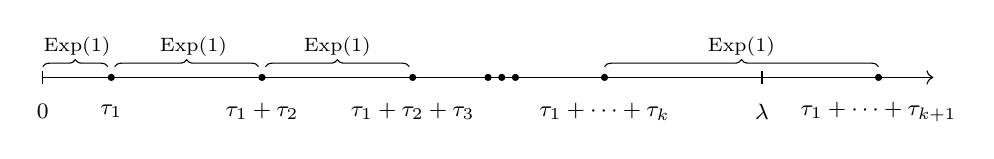
\begin{tikzpicture}[scale=0.87]
%\draw[help lines, color=gray!30, dashed] (-4.9,-4.9) grid (4.9,4.9);
\draw[->] (0,0)--(13,0) node[right]{};
\draw (0,-0.1)--(0,0.1) node[above]{};
\node () at (0.0,-0.5) {\footnotesize{$0$}};
\node (n0) at (0.0,0.3) {};



\fill (1,0)  circle[radius=1.5pt];
\node (n1) at (1,-0.5) {\footnotesize{$\tau_1$}};
\node (n1b) at (0.95,0.3) {};
\node (n1c) at (1.05,0.3) {};


\fill (3.2,0)  circle[radius=1.5pt];
\node () at (3.2,-0.5) {\footnotesize{$\tau_1+\tau_2$}};
\node (n2b) at (3.15, 0.3) {};
\node (n2c) at (3.25, 0.3) {};


\fill (5.4,0)  circle[radius=1.5pt];
\node (n3) at (5.4,-0.5) {\footnotesize{$\tau_1+\tau_2+\tau_3$}};
\node (n3b) at (5.35,0.3) {};
\node (n3c) at (5.45,0.3) {};

\fill (6.5,0)  circle[radius=1.5pt];
\fill (6.7,0)  circle[radius=1.5pt];
\fill (6.9,0)  circle[radius=1.5pt];




\fill (8.2,0)  circle[radius=1.5pt];
\node at (8.2,-0.5) {\footnotesize{$\tau_1+\cdots+\tau_k$}};
\node (nk) at (8.2,0.3) {};


\fill (12.2,0)  circle[radius=1.5pt];
\node at (12.2,-0.5) {\footnotesize{$\tau_1+\cdots+\tau_{k+1}$}};
\node (nk1) at (12.2,0.3) {};

\draw[thick] (10.5,-0.1)--(10.5,0.1) node[above]{};
\node at (10.5,-0.5) {\footnotesize{$\lambda$}};

\draw[decoration={brace }, decorate] (n0.south) -- (n1b.south) node {};

\draw[decoration={brace }, decorate] (n1c.south) -- (n2b.south) node {};



\draw[decoration={brace }, decorate] (n2c.south) -- (n3b.south) node {};


\draw[decoration={brace }, decorate] (nk.south) -- (nk1.south) node {};



\node at (0.5,0.45)  {\scriptsize{Exp$(1)$}};
\node at (2.2,0.45)  {\scriptsize{Exp$(1)$}};

\node at (4.3,0.45)  {\scriptsize{Exp$(1)$}};

\node at (10.2,0.45)  {\scriptsize{Exp$(1)$}};

\end{tikzpicture}
\caption{Renewal process and the Poisson distribution, see description in the text.}
\label{rys2-Poisson}
\end{figure}


Count the number $ N $ of $ \sigma_j $ points falling into the interval
$(0,\lambda]$;

\begin{equation}\label{e:Npoi}
N=\left\{
\begin{array}{ccc}
\max\{i\geq 1:\tau_1+\cdots+\tau_i\le \lambda\} & \textrm{ if } &\tau_1\le \lambda, \\[9pt]
0 &\textrm{ if }  &\tau_1>\lambda.
\end{array}
\right.
\end{equation}

\end{frame}



\begin{frame}{Poisson Poi($\lambda$)}


\begin{myProp} We have
$$N\eqdistr {\rm Poi}(\lambda).$$
\end{myProp}

\begin{proof}
\par\pause
We have $\Prob(N=0)=\Prob(\tau_1> \lambda)=e^{-\lambda}$. Moreover,
note the following equivalence
$$\{N\le k\}=\left\{\sum_{j=1}^{k+1}\tau_j> \lambda\right\}.$$
\noindent
Since (see \eqref{eq:tail_Erlang})
$$\Prob\left(\sum_{j=1}^{k+1}\tau_j>x\right)=
e^{-  x}\left(1+x+\frac{x^2}{2!}+\cdots+\frac{x^k}{k!}\right).$$
\end{proof}
\end{frame}



\begin{frame}{Poisson Poi($\lambda$)}


We have
\begin{align*}
\Prob(N=k)&=\Prob(\{N\le k\})-\Prob(\{N\le k-1\})\\
&= \Prob\left(\sum_{j=1}^{k+1}\tau_j>\lambda\right)-\Prob\left(\sum_{j=1}^{k}\tau_j>\lambda\right)\\
&= \frac{\lambda^k}{k!}e^{-\lambda}.\tag*{$\square$}
\end{align*}

\end{frame}




\begin{frame}{Poisson Poi($\lambda$)}
Based on the above, we have following procedure for sampling Poi($\lambda$):

\begin{algorithm}[H]
\index{algorithm!DP}
\caption{DP; generating $X\sim\mbox{Poi}(\lambda)$}
\label{alg:DP1}
\begin{algorithmic}[1]
\Require $\lambda>0$
\Ensure $X\sim\mbox{Poi}(\lambda)$
\State $X=0$
\State Generate $U\sim \calU[0,1)$
\State $S=-\log(U)$
\While  {$S<\lambda$}
\State Generate $U\sim \calU[0,1)$
\State  $Y=-\log(U)$
\State  $S=S+Y$
\State  $X=X+1$
\EndWhile
\State \Return $X$
\end{algorithmic}
\end{algorithm}

\end{frame}




\begin{frame}{Poisson Poi($\lambda$)}


Algorithm DP  can be further simplified using the following calculations.
If  $\tau_1> \lambda$,  then  $-\log U_1< \lambda$,
which is equivalent to $U_1< \exp(-\lambda)$. Thus,
\begin{eqnarray*}
N&=&\max\{n\ge0:\tau_1+\cdots+\tau_n\le \lambda\}\\
&=&\max\{n\ge0:(-\log U_1)+\cdots +(-\log U_n)\le \lambda\}\\
&=&\max\{n\ge0: \log \prod_{i=1}^nU_i\ge -\lambda\}\\
&=&\max\{n\ge0: \prod_{i=1}^nU_i\ge e^{-\lambda}\}\;.\label{eq:2Poisson}
\end{eqnarray*}
In the above, the  convention is that if $ n = $ 0, then
$\tau_1+\cdots+\tau_n=0$ (and  $\prod_{i=1}^0u_i=1$).
\end{frame}







\end{document}




\begin{frame}{Sequence of random numbers — formal definitions}
\begin{block}{On $[0,1)$}
A sequence $(U_j)_{j\ge 1}$ is a \textsl{sequence of random numbers} on $[0,1)$ if:
\begin{enumerate}
  \item[i)] Each $U_j$ has the uniform distribution $\calU[0,1)$, i.e.
  \[
    \Prob(U_j \le t) =
    \begin{cases}
      0 & t<0,\\
      t & 0\le t<1,\\
      1 & t\ge 1,
    \end{cases}
  \]
  \item[ii)] $U_1,U_2,\ldots$ are i.i.d., i.e., for $n\ge 1$,
  \[
    \Prob(U_1\le t_1,\ldots,U_n\le t_n)=t_1\cdots t_n .
  \]
\end{enumerate}
\end{block}

\smallskip
\begin{block}{Random bits}
$(B_j)_{j\ge 1}$ is a sequence of random bits if
$\Prob(B_j=0)=\Prob(B_j=1)=\tfrac12$ and $B_1,B_2,\ldots$ are i.i.d., so for $n\ge 1$,
\[
  \Prob(B_1=b_1,\ldots,B_n=b_n)=2^{-n}.
\]
\end{block}
\end{frame}

\begin{frame}{Discrete alphabet $\{0,1,\ldots,M-1\}$}
\begin{block}{Uniform on a finite set}
A sequence $(Y_j)_{j\ge 1}$ is a sequence of random numbers on
$\{0,1,\ldots,M-1\}$ if for each $j$:
\begin{enumerate}
  \item[i)] $\Prob(Y_j=i)=\tfrac1M$ for $i=0,\ldots,M-1$,
  \item[ii)] $Y_1,Y_2,\ldots$ are i.i.d., hence for $n\ge 1$,
  \[
    \Prob(Y_1=y_1,\ldots,Y_n=y_n)=M^{-n}.
  \]
\end{enumerate}
\end{block}

\smallskip
\begin{block}{Two practical remarks}
\begin{itemize}
  \item Computers output grid values in $\{0,\tfrac1M,\ldots,\tfrac{M-1}{M}\}$ (often $M=2^k$).
  \item Any subsequence chosen by increasing indices $n_1<n_2<\cdots$ remains i.i.d.\ with the same distribution.
\end{itemize}
\end{block}
\end{frame}

\begin{frame}{Pseudorandom number generators (PRNG)}
\begin{block}{Definition (deterministic mechanism)}
A PRNG is a 5-tuple $(S,s_0,f,V,g)$:
\begin{itemize}
  \item $S$ — finite state space,
  \item $s_0\in S$ — \textsl{seed} (initial state),
  \item $s_{i+1}=f(s_i)$, \ $f:S\to S$ — state recursion,
  \item $V$ — finite output alphabet,
  \item $g:S\to V$ — output function; $u_i=g(s_i)$ is the generated \textsl{pseudorandom} sequence.
\end{itemize}
\end{block}

\smallskip
\begin{block}{Key properties}
\begin{itemize}
  \item Deterministic $\Rightarrow$ fully reproducible via the seed.
  \item The period length is at most $|S|$.
  \item Construction/testing aim: practical \emph{indistinguishability} from an i.i.d.\ $\calU[0,1)$ sequence.
\end{itemize}
\end{block}
\end{frame}


% =======================
% Random permutations
% =======================

\section{Random permutations}

\begin{frame}{Random permutations}
\begin{block}{Definition}
Let $\calS_n$ be the set of all permutations of $[n]=\{1,\ldots,n\}$.
A \textsl{random permutation} is a random element $\pi$ taking all values in
$\calS_n$ with equal probability $1/n!$:
\[
  \Prob(\pi = \sigma) = \tfrac{1}{n!}, \qquad \sigma \in \calS_n.
\]
Equivalently, $\pi$ has the uniform distribution on $\calS_n$, denoted
$\calU(\calS_n)$.
\end{block}

\begin{block}{Goal}
Generate $\pi$ so that each permutation of $\{1,\ldots,n\}$ occurs with probability $1/n!$.
\end{block}
\end{frame}


\begin{frame}{Fisher–Yates algorithm}
\begin{block}{Idea}
Use a sequence of i.i.d.\ uniform random numbers $U_1,U_2,\ldots,U_n \sim \calU[0,1)$
to build a uniformly random permutation.
\end{block}

\begin{algorithm}[H]
\caption{\textsf{Fisher–Yates} (Random permutation)}\label{alg:fisher-yates}
\begin{algorithmic}[1]
\Require Integer \( n \); sequence \( \bfu=(u_1,\ldots,u_n),\ u_i\in[0,1) \)
\Ensure Permutation of \( \{1,\ldots,n\} \)
\State $S[i]=i,\ i=1,\ldots,n$
\For{$i=n$ downto $1$}
  \State $k=1+\lfloor i\,u_i\rfloor$ \Comment{choose a random position}
  \State \textbf{Swap}($S[k],S[i]$)
\EndFor
\State \textbf{Return} $S$
\end{algorithmic}
\end{algorithm}

\begin{itemize}
  \item[] $\bullet$ Complexity $O(n)$. $\qquad$ $\bullet$ Each permutation has equal probability $1/n!$.
\end{itemize}
\end{frame}

% =======================
% PRNGs in Python (NumPy)
% =======================

\section{Pseudorandom generators in Python}

\begin{frame}[fragile]{NumPy and random number generation}
\begin{block}{Setup}
We use \texttt{Python 3.12.2} and \texttt{NumPy 1.26.4} for all examples.
\begin{lstlisting}[frame=none,numbers=none]
import numpy as np
from numpy.random import default_rng
\end{lstlisting}
The modern interface uses \texttt{default\_rng()}, introduced in NumPy~1.17.
It replaces the legacy \texttt{np.random.rand()} (MT19937) API.
\end{block}

\begin{block}{Example}
\begin{lstlisting}[frame=none,numbers=none]
from numpy.random import default_rng, PCG64, MT19937
prng_pcg64   = default_rng(PCG64(seed=31415))
prng_mt19937 = default_rng(MT19937(seed=31415))

print(prng_pcg64.random(4))
print(prng_mt19937.random(4))
\end{lstlisting}
\end{block}

\begin{itemize}
  \item \texttt{default\_rng()} allows explicit choice of PRNG and seed.
  \item Without a seed, randomness comes from system entropy.
\end{itemize}
\end{frame}

\begin{frame}[fragile]{Available PRNG algorithms in NumPy}
\begin{block}{Main generators}
\begin{itemize}
  \item \texttt{PCG64} — default; period \(2^{128}\); excellent statistical quality.
  \item \texttt{Philox} — counter-based; period \(2^{256}-1\); parallel-friendly.
  \item \texttt{SFC64} — lightweight, very fast; period \(2^{255}\).
  \item \texttt{MT19937} — legacy 32-bit Mersenne Twister; period \(2^{19937}-1\).
\end{itemize}
\end{block}

\begin{block}{Basic usage}
\begin{lstlisting}[frame=none,numbers=none]
rng = default_rng(10)
rng.random(3)
rng.integers(0, 10, 5)
rng.permutation([1,2,3,4,5])
rng.normal(0, 1, 5)
\end{lstlisting}
\end{block}

\begin{block}{Note}
\texttt{PCG64} is recommended for new applications.
\end{block}
\end{frame}



% =======================
% Simple generators: historical perspective
% =======================

\section{Simple generators: historical perspective}

\begin{frame}{Linear congruential generators (LCGs)}
\begin{block}{Definition}
A linear congruential generator (LCG) produces
\[
x_{n+1} = (a x_n + c) \bmod M, \qquad
u_n = x_n / M.
\]
Parameters:
\[
M>0,\quad 0\le a<M,\quad 0\le c<M,\quad 0\le x_0<M.
\]
\end{block}

\begin{itemize}
  \item Period $\le M$; maximal period if
    \begin{enumerate}
      \item $c$ coprime with $M$,
      \item $a-1$ divisible by all prime factors of $M$,
      \item if $4\mid M$, then $a=1\bmod 4$.
    \end{enumerate}
  \item Historically popular:
    \[
      M=2^{31}-1,\ a=7^5,\ c=0.
    \]
  \item Simple and fast but poor randomness in high dimensions.
\end{itemize}
\end{frame}

\begin{frame}{Beyond simple LCGs}
\begin{block}{Generalized linear congruential generator (GLCG)}
\[
x_n = (a_1x_{n-1}+a_2x_{n-2}+\cdots+a_kx_{n-k}+c)\bmod M.
\]
If $M$ is prime and parameters are chosen carefully, period can reach $M^k$.
\end{block}

\begin{block}{L'Ecuyer combined generator}
Combines two recurrences:
\[
\begin{aligned}
x_n &= (A_1x_{n-2}-A_2x_{n-3}) \bmod M_1,\\
y_n &= (B_1y_{n-1}-B_2y_{n-3}) \bmod M_2,\\
z_n &= (x_n - y_n) \bmod M_1,\\
u_n &=
  \begin{cases}
  z_n / (M_1+1), & z_n>0,\\
  M_1/(M_1+1), & \text{otherwise.}
  \end{cases}
\end{aligned}
\]
Achieves very long period ($\approx 2^{191}$) and good statistical quality.
\end{block}
\end{frame}

\begin{frame}{Bitwise generators}
\begin{block}{Key operations}
Bitwise XOR ($\oplus$), left/right shifts ($\ll,\gg$) applied to $n$-bit registers.
\end{block}

\begin{block}{Examples}
\begin{itemize}
  \item \textbf{LFSR:} $x_i = (a_1x_{i-1}\oplus \cdots \oplus a_kx_{i-k})$ — maximal period $2^k-1$ with good tap choices.
  \item \textbf{Blum–Blum–Shub (BBS):} $x_{i+1}=x_i^2\bmod M$, $M=pq$; secure but slow.
  \item \textbf{Shift–XOR (SXR):} $x_{i+1}=(x_i\oplus(x_i\ll a))\oplus(x_i\gg b)$ — efficient 32/64-bit generator.
\end{itemize}
\end{block}

\begin{block}{Summary}
Early PRNGs (LCG, GLCG) were educational and lightweight.
Modern generators (e.g., PCG, Philox) build on these ideas but overcome short periods and poor lattice structure.
\end{block}
\end{frame}

\section{Testing pseudorandom number generators (PRNGs)}


\begin{frame}{Notation and motivation}
\begin{itemize}
  \item $U$: random variable $\calU[0,1)$.
  \item $Y$: random variable $\calU(\bar{M})$, i.e.\ uniform on $\{0,\ldots,M-1\}$.
  \item $B$: random bit, $\calU[\{0,1\}]$.
\end{itemize}

\begin{block}{Motivation}
Different statistical tests use different data types:
\begin{itemize}
  \item numbers in $[0,1)$,
  \item integers in $\{0,\ldots,M-1\}$,
  \item or sequences of bits.
\end{itemize}
We must reliably convert between these forms.
\end{block}
\end{frame}

\begin{frame}{Converting numbers between formats}
\begin{block}{Continuous $\leftrightarrow$ discrete}
From $u_i\in[0,1)$ to $\{0,\ldots,M-1\}$:
\[
y_i = \lfloor M u_i \rfloor .
\]
From $y_i$ to $u_i$:
\[
u_i = y_i / M .
\]
\end{block}

\begin{block}{Example (Visual Basic PRNG)}
\[
x_i = (1140671485\,x_{i-1} + 12829163) \bmod 2^{24}, \qquad
u_i = x_i / 2^{24}.
\]
Each $u_i$ has $2^{24}$ possible values,
so it is natural to convert via $y_i=\lfloor2^{24}u_i\rfloor$.
\end{block}
\end{frame}

\begin{frame}{Converting to bits and grouping vectors}
\begin{block}{Caution when converting to bits}
Simple mapping
\[
b_i =
\begin{cases}
0,&u_i<0.5,\\
1,&u_i\ge 0.5
\end{cases}
\]
uses only the most significant bit of $u_i$.
Better: first compute $y_i=\lfloor M u_i\rfloor$ (with $M=2^k$),
then use the full binary expansion of $y_i$.
\end{block}


\end{frame}

\begin{frame}{Grouping numbers into vectors}
Given $n = mr$ elements of a sequence, group them into $r$ $m$-dimensional vectors.
\begin{itemize}
 \item  From  $u_i \in [0,1)$ we construct $\bfu_j \in [0,1)^m$:
\[
\bfu_j = (u_{(j-1)m+1}, \ldots, u_{jm}), \quad j=1,\ldots,r.
\]

\item  From  $y_i \in \{0,\ldots,M-1\}$ we construct $\bfy_j \in \{0,\ldots,M-1\}^m$:
\[
\bfy_j = (y_{(j-1)m+1}, \ldots, y_{jm}), \quad j=1,\ldots,r.
\]
\item From  $b_i \in \{0,1\}$ we construct   $\bfb_j \in \{0,1\}^m$:
\[
\bfb_j = (b_{(j-1)m+1}, \ldots, b_{jm}), \quad j=1,\ldots,r.
\]
\end{itemize}

\begin{itemize}
  \item Such grouping enables testing of $m$-dimensional uniformity.
  \item Used in tests like the \textsl{serial test} or \textsl{spectral test}.
\end{itemize}
\end{frame}

\subsection{The concept of $p$-value}
% =======================
% p-value concept
% =======================

\begin{frame}{The concept of $p$-value}
We test randomness using a statistic \(T\) computed from a generated sequence.
\[
\calH_0: \text{the sequence is i.i.d.\ uniform.}
\]

For observed \(T(\text{obs})\), the $p$-value is the probability (under $\calH_0$)
of obtaining a value of $T$ at least as extreme as $T(\text{obs})$.

\begin{itemize}
 \item Right-tail test: \(p = 1 - G(T(\text{obs}))\)
 \item Left-tail test: \(p = G(T(\text{obs}))\)
 \item Two-sided (symmetric \(T\)): \(p = G(-T(\text{obs})) + 1 - G(T(\text{obs}))\)
\end{itemize}

\medskip
\begin{itemize}
  \item Large $p \Rightarrow$  consistent with randomness (\(\calH_0\)).
  \item Very small $p \Rightarrow$  evidence against randomness.
\end{itemize}
\end{frame}

\begin{frame}{Example: frequency (monobit) test}
bits \(B_i\), define \(X_i = 2B_i - 1\) and \(S_n = X_1 + \cdots + X_n\).
Under $\calH_0$: \(S_n / \sqrt{n} \approx \mathcal{N}(0,1)\).

\[
T(\text{obs}) = \left| \frac{s_n}{\sqrt{n}} \right|, \quad
p = 2(1 - \Phi(T(\text{obs}))).
\]

\begin{center}
\begin{figure}[h]
 \centering
 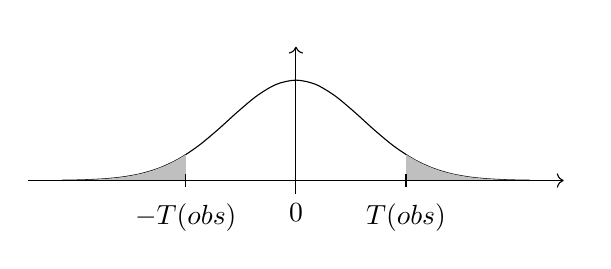
\begin{tikzpicture}[scale=0.85]
    % Draw the normal distribution curve
    \draw[domain=-3.5:3.5, smooth, variable=\x] plot ({\x}, {1.5*exp(-0.5*\x*\x)});

    % Shade the right tail area
    \fill[gray!50] (1.645,0) -- plot[domain=1.645:3.5, smooth, variable=\x] ({\x}, {1.5*exp(-0.5*\x*\x)}) -- (3.5,0) -- cycle;

    % Shade the left tail area
    \fill[gray!50] (-1.645,0) -- plot[domain=-1.645:-3.5, smooth, variable=\x] ({\x}, {1.5*exp(-0.5*\x*\x)}) -- (-3.5,0) -- cycle;

    % Label for the mean
    \node[below] at (0,-0.2) {$0$};

    % Label for the right critical value
    \node[below] at (1.645,-0.2) {$T(\text{obs})$};

    % Label for the left critical value
    \node[below] at (-1.645, -0.2) {$-T(\text{obs})$};

    % Axes
    \draw[->] (-4,0) -- (4,0) node[right] {};
    \draw[->] (0,-0.2) -- (0,2) node[above] {};

    \draw[-] (1.645,-0.1) -- (1.645,0.1) node[right] {};
    \draw[-] (-1.645,-0.1) -- (-1.645,0.1) node[right] {};


\end{tikzpicture}
\caption{
Density of standard normal $Z\sim \calN(0,1)$ random variable. Shaded area is equal to $p$-value $\Prob(|Z|\geq T(\text{obs}))$.
}\label{fig:normal_distr_two_sided}
\end{figure}




\end{center}

\begin{itemize}
  \item Two-sided test, using the half-normal distribution.
  \item Approximation valid for \(n \ge 30\); in practice \(n\) is usually much larger.
  \item Part of a family of tests based on random walks.
\end{itemize}
\end{frame}

\subsection{Two fundamental goodness-of-fit tests}
\begin{frame}{Two fundamental goodness-of-fit tests}
We use two general-purpose tests to assess the uniformity (and thus randomness) of PRNG output:
\begin{itemize}
  \item the \textbf{chi-square test}, and
  \item the \textbf{Kolmogorov–Smirnov (KS) test}.
\end{itemize}

\medskip
Example: three sets of $n=50$ numbers ($A$, $B$, $C$) are shown below.
The partition of $[0,1)$ is
\[
P_1=(0,0.15),\;
P_2=[0.15,0.35),\;
P_3=[0.35,0.6),\;
P_4=[0.6,0.8),\;
P_5=[0.8,1).
\]

\begin{center}
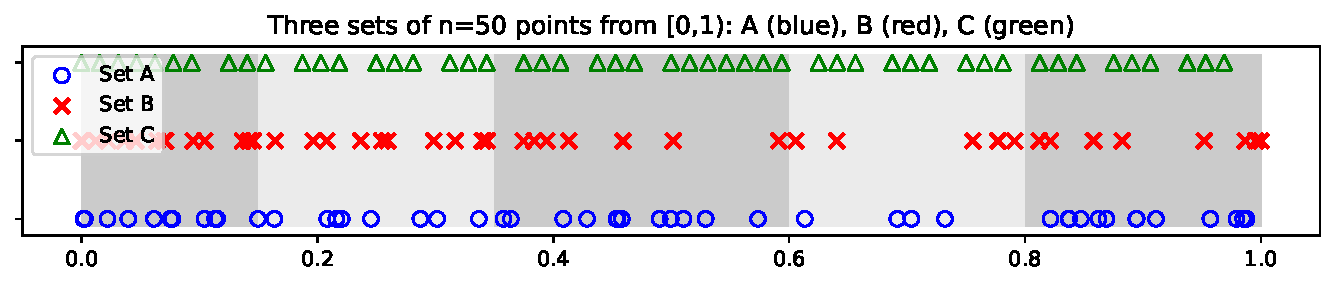
\includegraphics[width=0.8\linewidth]{figures_pdf/ch2_prng_sets_A_B_C_points_plot.pdf}
\end{center}

\begin{itemize}
  %\item Set $C$ originates from a quasirandom generator.
  \item Goal: determine whether sets $A$, $B$, and $C$ are consistent with uniform randomness.
\end{itemize}
\end{frame}

\subsection{Kolmogorov–Smirnov (KS) test}
% =======================
% Kolmogorov–Smirnov goodness-of-fit test
% =======================

\begin{frame}{Kolmogorov–Smirnov (KS) test}
We test whether $U_1,\ldots,U_n$ are distributed as $\calU[0,1)$.

Empirical c.d.f.:
\[
\hat{F}_n(t)=\frac{1}{n}\sum_{i=1}^n \ind(U_i\le t),
\qquad F(t)=t.
\]

Test statistic:
\[
D_n = \sup_{0\le t\le 1}|\hat{F}_n(t)-t|.
\]

If $U_i\sim\calU[0,1)$, then $\sqrt{n}D_n$ converges in distribution to
the \textsl{Kolmogorov distribution} $K(t)$:
\[
K(t)=\sum_{j=-\infty}^{\infty}(-1)^j e^{-2j^2t^2}.
\]
Critical values:
$\lambda_{0.1}=1.224$, $\lambda_{0.05}=1.358$, $\lambda_{0.01}=1.628$.
\end{frame}

\begin{frame}{Computation and $p$-value}
Order the sample: $U_{(1)}\le\cdots\le U_{(n)}$.

\[
D_n^+ = \max_i\!\left(\frac{i}{n}-U_{(i)}\right), \quad
D_n^- = \max_i\!\left(U_{(i)}-\frac{i-1}{n}\right),
\quad D_n=\max(D_n^+,D_n^-).
\]

$p$-value:
\[
p = 1 - K\!\left(\sqrt{n}D_n(\text{obs})
+ \frac{1}{6\sqrt{n}}
+ \frac{\sqrt{n}D_n(\text{obs})-1}{4n}\right).
\]
The correction improves small-$n$ accuracy
(see Vrbik, 1995).
\end{frame}

\begin{frame}{Example: sets $A$, $B$, $C$}
Empirical c.d.f.s for $A$, $B$, $C$
are compared with $F(t)=t$ for $\calU[0,1)$.

\[
D_n^A=0.1192,\quad D_n^B=0.2266,\quad D_n^C=0.0462.
\]
\[
p^A=44.17\%,\quad p^B=0.99\%,\quad p^C=99.97\%.
\]



\begin{center}
\begin{tabular}{ccc}
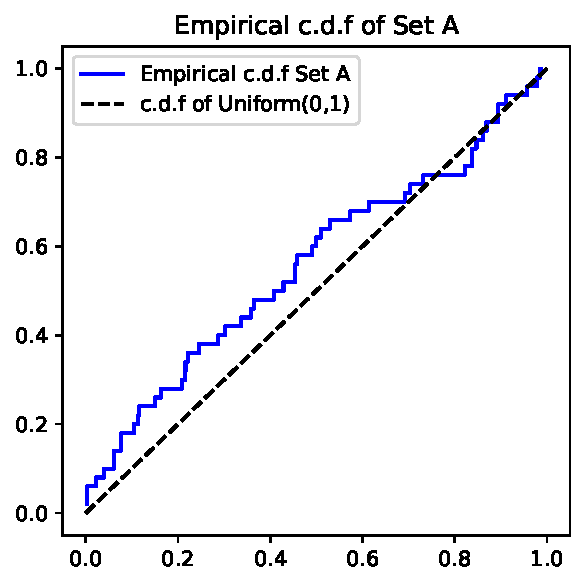
\includegraphics[width=0.25\linewidth]{figures_pdf/ch2_prng_sets_A_B_C_empCDF_of_setA.pdf}
&
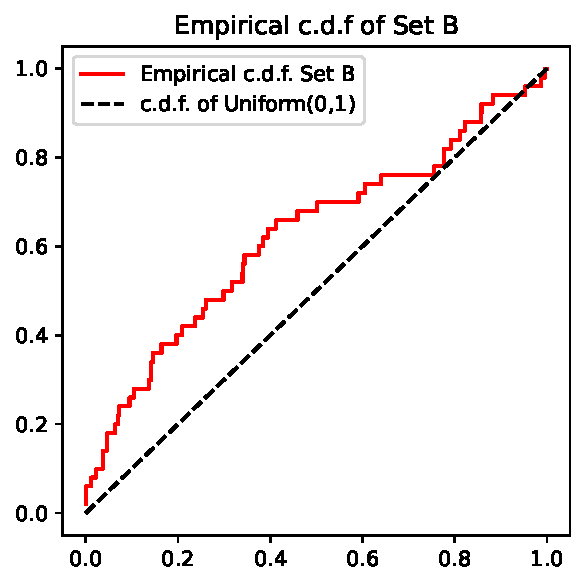
\includegraphics[width=0.25\linewidth]{figures_pdf/ch2_prng_sets_A_B_C_empCDF_of_setB.pdf} &
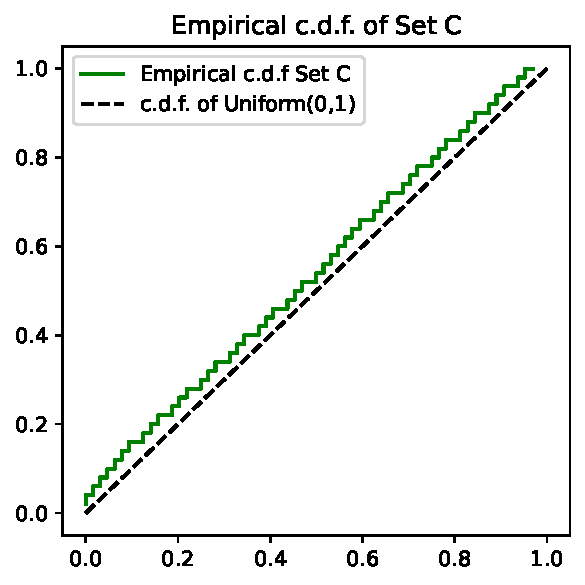
\includegraphics[width=0.25\linewidth]{figures_pdf/ch2_prng_sets_A_B_C_empCDF_of_setC.pdf}
\end{tabular}
\end{center}
\end{frame}

% =======================
% Chi-square goodness-of-fit
% =======================

\subsection{Chi-square goodness-of-fit (Pearson)}
\begin{frame}{Chi-square goodness-of-fit (Pearson)}
Multinomial setting: \(\mathrm{M}(r,p_1,\ldots,p_k)\).
Outcomes \(i=1,\ldots,k\) with probabilities \(p_i\); counts \(O_i\), expectations \(E_i=\Exp O_i=rp_i\).

\[
X_k^2=\sum_{i=1}^k \frac{(O_i-rp_i)^2}{rp_i}
      =\sum_{i=1}^k \frac{O_i^2}{rp_i}-r.
\]

As \(r\to\infty\): \(\;X_k^2 \convdistr \chi^2_{k-1}\).
For data: compute \(O_i\), then \(X_k^2\) and the \(p\)-value from \(\chi^2_{k-1}\).
\end{frame}

\begin{frame}{Using it for uniformity on \([0,1)\)}
Partition \( [0,1) \) into \(k\) bins \(P_i\) with lengths \(p_i=|P_i|\).
Given \(r\) samples, let \(O_i=\#\{u_j\in P_i\}\), then use
\[
X_k^2=\sum_{i=1}^k \frac{(O_i-rp_i)^2}{rp_i}, \qquad X_k^2 \approx \chi^2_{k-1}.
\]

\textbf{Rule of thumb:} each expected count \(\ge 5\):
\[
r \;\ge\; \left\lceil \frac{5}{\displaystyle \min_{1\le i\le k} p_i}\right\rceil.
\]

Notes:
\begin{itemize}
  \item Choice of \(k\), partition, and interpretation depends on application.
  \item For \(k\gg r\), prefer balls-and-boxes style tests.
\end{itemize}
\end{frame}

\begin{frame}{Example (sets \(A,B,C\); partition \(\calP\))}
Recall:
\begin{center}
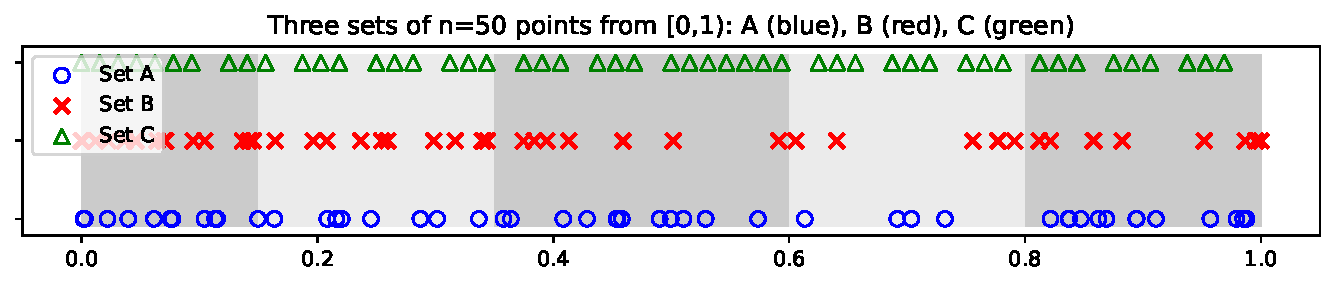
\includegraphics[width=0.6\linewidth]{figures_pdf/ch2_prng_sets_A_B_C_points_plot.pdf}
\end{center}

With \(k=5\) bins from  , \(r=50\) satisfies the rule (\(p_{\min}=0.15\Rightarrow 34\)).

\[
X_A^2(\text{obs})=7.32,\quad
X_B^2(\text{obs})=16.25,\quad
X_C^2(\text{obs})=0.24,
\]
\[
p^A=11.99\%,\quad p^B=0.27\%,\quad p^C=99.35\% \quad (\chi^2_4).
\]

Interpretation:
\begin{itemize}
  \item \(A\): not rejected (consistent with uniformity).
  \item \(B\): rejected (very small \(p\)).
  \item \(C\): not rejected; very large \(p\) .
\end{itemize}

For large \(k\): \(\chi^2_k \eqdistr Z_1^2+\cdots+Z_k^2\), so
$
\frac{\chi^2_k - k}{\sqrt{2k}} \convdistr \mathcal{N}(0,1).
$
\end{frame}


\subsection{Statistical test contd.}

% =======================
% Spacing test — definition
% =======================

\begin{frame}{Spacing test}
Fix $(\alpha,\beta] \subset (0,1]$, let $\delta=\beta-\alpha$.
Indices hitting the interval:
\[
\{i\ge1: U_i\in(\alpha,\beta]\}=\{S_1<S_2<\cdots\},\quad
C_1=S_1,\ C_j=S_j-S_{j-1}\ (j\ge2).
\]
Under $\calH_0$ ($U_i$ i.i.d.\ $\calU[0,1)$):
\[
\Prob(C=l)= (1-\delta)^{\,l-1}\,\delta,\qquad l=1,2,\ldots
\]
(geometric on $\{1,2,\ldots\}$, mean $1/\delta$, var $(1-\delta)/\delta^2$).

For a finite sample $U_1,\ldots,U_n$:
\[
\{i\le n: U_i\in(\alpha,\beta]\}=\{S_1<\cdots<S_K\},\quad
C_1=S_1,\ldots, C_K=S_K-S_{K-1}.
\]
Choose bins
\[
A_0=\{0\},\,A_1=\{1\},\ldots,A_{s-1}=\{s-1\},\ A_s=\{s,s+1,\ldots\},
\]
with
\[
s\ \ge\ \max\!\left\{5,\ \left\lceil \frac{5(1-\delta)}{\delta}\right\rceil\right\}.
\]
\end{frame}

% =======================
% Spacing test — chi-square
% =======================

\begin{frame}{Spacing test: chi-square implementation}
Expected bin probabilities:
\[
p_i=\delta(1-\delta)^i\ (i=0,\ldots,s-1),\qquad
p_s=1-\sum_{i=0}^{s-1}p_i.
\]
Observed counts:
\[
O_i=\#\{j: C_j\in A_i\},\quad i=0,\ldots,s,\qquad \text{total }K.
\]
Test statistic:
\[
X^2(\text{obs})=\sum_{i=0}^{s}\frac{(O_i-Kp_i)^2}{Kp_i}\ \approx\ \chi^2_s\quad(\calH_0).
\]
Notes:
\begin{itemize}
  \item Sensitivity to bin choice—coarse vs.\ fine \(A_i\) may reveal/hide structure.
  \item Rule of thumb: ensure all \(Kp_i\gtrsim 5\).
\end{itemize}
\end{frame}

% =======================
% Serial test (incl. frequency tests)
% =======================
\begin{frame}{Serial test \((m,L)\) and special cases}
Partition \([0,1)^m\): split each axis into \(L\) equal parts; total \(k=L^m\) boxes.
Group \(n=mr\) values into \(r\) vectors
\[
\bfu_j=(u_{(j-1)m+1},\ldots,u_{jm})\in[0,1)^m,\quad j=1,\ldots,r.
\]


\begin{figure}[h]
\begin{center}6
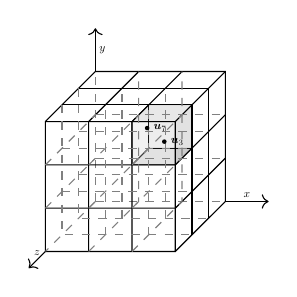
\begin{tikzpicture}[scale=0.55, every node/.style={scale=0.75}, transform shape]
  \draw[fill=gray!20, opacity=0.6] (3,3,3) -- (2,3,3) -- (2,2,3) -- (3,2,3); % przod
  \draw[fill=gray!45, opacity=0.6] (3,3,3) -- (2,3,3) -- (2,3,2) -- (3,3,2); % gora
  \draw[fill=gray!60, opacity=0.9] (3,3,3) -- (3,3,2) -- (3,2,2) -- (3,2,3); % prawy bok
  \draw[fill=gray!30, opacity=0.6] (3,2,3) -- (2,2,3) -- (2,2,2) -- (3,2,2); % dol
  \draw[fill=gray!10, opacity=0.5] (2,3,3) -- (2,3,2) -- (2,2,2) -- (2,2,3); % lewy  bok
  \draw[fill=gray!15, opacity=0.8] (3,3,2) -- (2,3,2) -- (2,2,2) -- (3,2,2); % przod



  \draw (3,0,0) coordinate (x) |- (0,3,0) coordinate [midway] (h) coordinate (y) -- (0,3,3) coordinate (a) -- (0,0,3) coordinate (z) -- (3,0,3) edge (x) -- (3,3,3) coordinate (v) edge (h)
  -- (a)  ;

  \draw [dashed, color=gray] (0,0,0) coordinate (o) edge (x) edge (y) -- (z);

  %\draw[->,color=red] (x) -- (o);


  \draw (1,0,3) -- (1,3,3) -- (1,3,0);
  \draw (2,0,3) -- (2,3,3) -- (2,3,0);

  \draw (0,3,1) -- (3,3,1) -- (3,0,1);
  \draw (0,3,2) -- (3,3,2) -- (3,0,2);


  \draw (0,1,3) -- (3,1,3) -- (3,1,0);
  \draw (0,2,3) -- (3,2,3) -- (3,2,0);


  \draw [dashed, color=gray] (1,0,1) -- (1,3,1) ;
  \draw [dashed, color=gray] (1,0,2) -- (1,3,2) ;

  \draw [dashed, color=gray] (2,0,1) -- (2,3,1);
  \draw [dashed, color=gray] (2,0,2) -- (2,3,2) ;

  \draw [dashed, color=gray] (0,3,1) -- (0,0,1) -- (3,0,1);
  \draw [dashed, color=gray] (0,3,2) -- (0,0,2) -- (3,0,2);

  \draw [dashed, color=gray] (1,0,3) -- (1,0,0) -- (1,3,0);
  \draw [dashed, color=gray] (2,0,3) -- (2,0,0) -- (2,3,0);

  \draw [dashed, color=gray] (0,1,0) -- (3,1,0);
  \draw [dashed, color=gray] (0,1,1) -- (3,1,1);
  \draw [dashed, color=gray] (0,1,2) -- (3,1,2);

  \draw [dashed, color=gray] (0,2,0) -- (3,2,0);
  \draw [dashed, color=gray] (0,2,1) -- (3,2,1);
  \draw [dashed, color=gray] (0,2,2) -- (3,2,2);

  \draw [dashed, color=gray] (1,1,3) -- (1,1,0);
  \draw [dashed, color=gray] (2,1,3) -- (2,1,0);

  \draw [dashed, color=gray] (1,2,3) -- (1,2,0);
  \draw [dashed, color=gray] (2,2,3) -- (2,2,0);

  \draw [dashed, color=gray] (0,1,3) -- (0,1,0) ;
  \draw [dashed, color=gray] (0,2,3) -- (0,2,0) ;

  \node [circle, minimum size=4pt, inner sep=0pt, fill, label=0:$\bfu_3$] at (2.4, 2.19, 2.1) {};
  \node [circle, minimum size=4pt, inner sep=0pt, fill, label=0:$\bfu_7$] at (2.1, 2.6, 2.35) {};
  \draw [->] (x) -- +(1pt,0,0) node [midway,above] {$x$};
  \draw [->] (y) -- +(0,1pt,0) node [midway,right] {$y$};
  \draw [->] (z) -- +(0,0,1pt) node [midway,above] {$z$};
  %\draw [color=brown] (v) -- ++(0,0,-1) coordinate (d) -- ++(-1,0,0) coordinate (e) -- ++(0,0,1) |- ++(1,-1,0) coordinate [midway] (f) -- ++(0,0,-1) coordinate (g) -- (d);
  %\draw [dashed] (e) -- ++(0,-1,0) coordinate (c) edge (f) -- (g);
  %\node [label=45:C] at (c) {};
 \end{tikzpicture}
\caption{Sample cube $[0,1)^m, m=3$, each side split into $L=3$ segments obtaining $k=L^3=27$
smaller sub-hypercubes. Sample points  $\bfu_3=(0.8, 0.73, 0.7)$ and $\bfu_7=(2.1, 2.6, 2.35)$ are presented together with the corresponding box
$A_{2,2,2}=\left\{(v_1,v_2,v_3): v_i\in\left({2\over 3},1\right), i=1,2,3\right\}$, or correspondingly $\bfy_3=\bfy_7=(2,2,2)$ and $A'_{2,2,2}=(2,2,2)$ (see description in the text).}
\label{fig:cube_bins}
\end{center}
\end{figure}
\end{frame}

\begin{frame}{Serial test \((m,L)\) and special cases}
The sub-hypercubes:
\begin{equation}\label{eq:sub-hypercubes}
A_{q_1,\ldots,q_m}=\left\{(v_1,\ldots,v_m): v_i \in \left[\frac{q_i}{L},\frac{q_i+1}{L}\right), \, i=1,\ldots,m\right\},
\end{equation}
where \(q_i \in \{0,\ldots,L-1\}\).
 Count the vectors:
\[
O_{q_1,\ldots,q_m} = \#\{i : \bfu_i \in A_{q_1,\ldots,q_m}\}, \quad (q_1,\ldots,q_m) \in \{0,\ldots,L-1\}^m.
\]
With \(k = L^m\), compute the chi-square statistic:
\[
X^2(\text{obs}) = \sum_{(q_1,\ldots,q_m) \in \{0,\ldots,L-1\}^m} \frac{(O_{q_1,\ldots,q_m} - r/k)^2}{r/k}.
\]
 Under the null hypothesis \(\calH_0\) (that the sequence is sampled from \(\calU[0,1)\)), for large \(r\), \(X^2\) is approximately chi-square distributed with \(k-1\) degrees of freedom.
\end{frame}

\begin{frame}{Serial test \((m,L)\) and special cases}
Partition \([0,1)^m\): split each axis into \(L\) equal parts; total \(k=L^m\) boxes.
Group \(n=mr\) values into \(r\) vectors
\[
\bfu_j=(u_{(j-1)m+1},\ldots,u_{jm})\in[0,1)^m,\quad j=1,\ldots,r.
\]
Counts per box \(O_{q_1,\ldots,q_m}\) with expected \(r/k\).
\[
X^2(\text{obs})=\sum_{(q_1,\ldots,q_m)}\frac{(O_{q_1,\ldots,q_m}-r/k)^2}{r/k}\ \approx\ \chi^2_{k-1}.
\]
Guidelines (Holst; L’Ecuyer et al.):
\begin{itemize}
  \item Fixed \(k\), \(r\to\infty\): \(X^2\to\chi^2_{k-1}\).
  \item \(r,k\to\infty\), \(r/k\to\gamma\in(0,\infty)\): standardized \(X^2\Rightarrow\calN(0,1)\);
        prefer \(0<\gamma<5\); for \(\gamma\ge5\) the \(\chi^2\) approx.\ improves.
\end{itemize}
Special cases:
\begin{itemize}
  \item \(m=1\) (frequency test): \(k=L\), \(O_i=\#\{j:y_j=i\}\), \(X^2=\sum_{i=0}^{k-1}\frac{(O_i-n/k)^2}{n/k}\).
  \item \(m=2\) (frequency of pairs): \(k=L^2\), \(O_{s,t}=\#\{j:(y_{2j-1},y_{2j})=(s,t)\}\),
        \(X^2=\sum_{s,t}\frac{(O_{s,t}-r/k)^2}{r/k}\).
\end{itemize}
\end{frame}

% =======================
% Tests based on "balls and boxes" scheme
% =======================

\subsection{Tests based on ``balls and boxes'' schemes}

\begin{frame}{Balls and boxes: setup}
We place \(r\) balls into \(k\) boxes, independently, with \(\Prob(\text{box }i)=p_i=1/k\) under \(\calH_0\).
This scheme underlies multiple tests of uniformity/independence.



\begin{center}
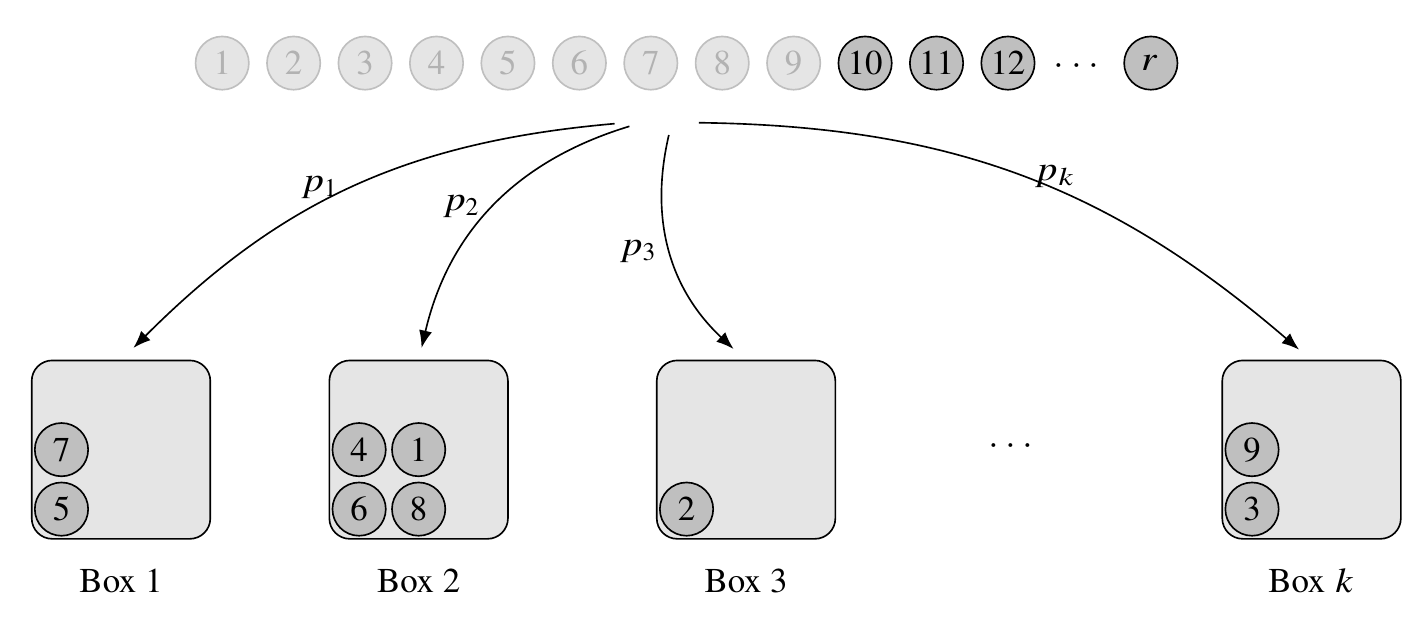
\includegraphics[width=0.8\linewidth]{pics/ball_into_boxes.png}
\end{center}
\end{frame}

% -----------------------

\begin{frame}{Birthday problem and collisions}
Birthday problem: \(k=365\) boxes (days), \(r\) balls (people).
\[
\Prob(\text{all unique})=\frac{(365)_r}{365^r},\qquad
p=1-\frac{(365)_r}{365^r}=1-\prod_{j=1}^{r-1}\Bigl(1-\frac{j}{365}\Bigr).
\]
General \(k\):
\[
p_{k,r}=1-\prod_{j=1}^{r-1}\Bigl(1-\frac{j}{k}\Bigr)\approx 1-\exp\!\left(-\frac{r^2}{2k}\right).
\]


\end{frame}

% -----------------------

\begin{frame}{Collision test (definition and approximation)}
Define the \textbf{number of collisions} \(C_{k,r}\): times a ball hits an already occupied box.
Then \(p_{k,r}=\Prob(C_{k,r}>0)\).
Given \(r\) balls, \(k\) boxes, the exact distribution of \(C_{k,r}\) is
\[
\Prob(C_{k,r}=c)=\frac{k(k-1)\cdots(k-r+c+1)}{k^r}\,S_2(r,r-c),\qquad c=0,1,\ldots,
\]
where \(S_2(\cdot,\cdot)\) are Stirling numbers of the second kind (counts of set partitions).

\medskip
\pause
Poisson approximation (no proof here): if \(r,k\to\infty\) with \(\tfrac{r^2}{2k}\to\lambda\in(0,\infty)\),
\[
\Prob(C_{k,r}=c)\ \to\ \frac{\lambda^c}{c!}e^{-\lambda},\qquad c=0,1,\ldots
\]
Mean comparison:
\[
\lambda\ \approx\ \frac{r^2}{2k},\qquad
\Exp C_{k,r}=r-k\Bigl(1-(1-\tfrac1k)^r\Bigr).
\]
Example: \(k=2^{20}, r=2^{14}\): \(r^2/(2k)=128\) vs.\ \(\Exp C_{k,r}=127.3282\).
\end{frame}

% -----------------------







\end{document}

